\documentclass[12pt]{scrartcl}

\usepackage[T1]{fontenc}
\usepackage[utf8]{inputenc}
\usepackage{amsmath}
\usepackage{amsfonts}
\usepackage{amssymb}
\usepackage{amsbsy}
\usepackage{graphicx}
\usepackage{float}
\usepackage{array}
\usepackage{booktabs}
\usepackage{multirow}
\usepackage{bm}
\usepackage{verbatim}
\usepackage[english]{babel}
\usepackage{color}
\usepackage{url}
\usepackage{fancybox}
\usepackage[stable]{footmisc}
\usepackage[format=plain,labelfont=bf]{caption}
\usepackage{fancyhdr}
\usepackage{natbib}
\usepackage{calc}
\usepackage{textcomp}
\usepackage[pdftex,pdfborder={0 0 0}]{hyperref}
\usepackage{pdfpages}
\usepackage{tikz}
\usetikzlibrary{shapes,backgrounds,fit,positioning}
\usepackage{mathtools}
\renewcommand*{\familydefault}{\sfdefault}

% Margins
\addtolength{\textheight}{1.0cm}
\addtolength{\oddsidemargin}{-0.5cm}
\addtolength{\evensidemargin}{-0.5cm}
\addtolength{\textwidth}{1.0cm}
\parindent=0em

% New math commands
\newcommand{\overbar}[1]{\mkern 1.5mu\overline{\mkern-1.5mu#1\mkern-1.5mu}\mkern 1.5mu}
\DeclareMathOperator{\diag}{diag}
\DeclareMathOperator{\Diag}{Diag}
\DeclareMathOperator{\tr}{tr}
\DeclareMathOperator{\Cov}{Cov}
\DeclareMathOperator{\Cor}{Cor}
\newcommand\independent{\protect\mathpalette{\protect\independenT}{\perp}}
\def\independenT#1#2{\mathrel{\setbox0\hbox{$#1#2$}%
\copy0\kern-\wd0\mkern4mu\box0}}

% Appropriate font for \mathcal{}
\DeclareSymbolFont{cmmathcal}{OMS}{cmsy}{m}{n}
\DeclareSymbolFontAlphabet{\mathcal}{cmmathcal}

% Set subscript and superscripts positions
\everymath{
\fontdimen13\textfont2=5pt
\fontdimen14\textfont2=5pt
\fontdimen15\textfont2=5pt
\fontdimen16\textfont2=5pt
\fontdimen17\textfont2=5pt
}

% Bibliography style
\setlength{\bibsep}{1pt}

% Part
\renewcommand\partheadstartvskip{\clearpage\null\vfil}
\renewcommand\partheadmidvskip{\par\nobreak\vskip 20pt\thispagestyle{empty}}
\renewcommand\partheadendvskip{\vfil\clearpage}
\renewcommand\raggedpart{\centering}

\begin{document}

\title{\vspace{-1.2cm}Normalized Interpolated Convolution from an Adaptive Subgrid}
\author{Benjamin Ménétrier}
\date{Last update: \today\vspace{-0.5cm}}

\thispagestyle{empty}

\maketitle

\begin{center}
Documentation for the code "BUMP", distributed under the CeCILL-C license.\\
Copyright \copyright 2015-... UCAR, CERFACS, METEO-FRANCE and IRIT
\end{center}

\tableofcontents

\clearpage

\section{Introduction}
The application of a localization matrix $\mathbf{C} \in \mathbb{R}^{n \times n}$ to a vector $\mathbf{x} \in \mathbb{R}^n$ requires $n^2$ multiplications and $n(n-1)$ additions, which can too expensive for large systems. If the localization functions inside $\mathbf{C}$ are compactly supported, then $\mathbf{C}$ has a lot of zeros and the cost is reduced. However in this case, the cost increases with the size of the localization functions support: the larger the support, the larger the number of points involved and therefore the cost.\\
$  $\\
The idea of the NICAS method is to apply an equivalent localization operator on a subgrid $\mathcal{G}^s$ that contains a subset of $n^s$ points of the full grid $\mathcal{G}^f$, with $n^s \ll n$. We define the localization matrix $\mathbf{C}^s \in \mathbb{R}^{n^s \times n^s}$ and the linear interpolation operator $\mathbf{S} \in \mathbb{R}^{n \times n^s}$. The NICAS localization matrix is given by:
\begin{align}
\label{eq:nicas}
\widetilde{\mathbf{C}} = \mathbf{N} \mathbf{S} \mathbf{C}^s \mathbf{S}^\mathrm{T} \mathbf{N}^\mathrm{T}
\end{align}
where $\mathbf{N} \in \mathbb{R}^{n \times n}$ is a diagonal operator, which ensures that $\widetilde{\mathbf{C}}$ is normalized (i.e. $\widetilde{C}_{ii} = 1$). Indeed, even if $\mathbf{C}^s$ is normalized, $\mathbf{S} \mathbf{C}^s \mathbf{S}^\mathrm{T}$ is not normalized.\\
$  $\\
The ARPEGE model is the operational global model at Météo-France. Most illustrations are drawn from preliminary experiments that have been conducted with ARPEGE on a low-resolution grid (truncation TL149) with 106 levels. Scaling experiments also use a higher-resolution grid (truncation TL399).

\section{Convolution subgrid}
The choice of the subgrid is directly linked to the interpolation methods used in $\mathbf{S}$. Since a full 3D interpolation might be hard to compute and to apply in a geophysical model, we split $\mathbf{S}$ into three operators:
\begin{align}
\mathbf{S} = \mathbf{S}^h \mathbf{S}^v \mathbf{S}^s
\end{align}
To describe $\mathbf{S}^h$, $\mathbf{S}^v$ and $\mathbf{S}^s$, it is easier to look at the grids they are interpolating to:
\begin{itemize}
\item $\mathcal{G}^f$ is the full grid, with a set $\mathcal{S}^c_0$ of $n^c_0$ horizontal points and a set $\mathcal{S}^l_0$ of $n^l_0$ levels,
\item $\mathcal{G}^h$ is the first intermediate subgrid, with a subset $\mathcal{S}^c_1$ of $n^c_1$ horizontal points ($n^c_1 \le$ $n^c_0$) and the set $\mathcal{S}^l_0$ of $n^l_0$ levels,
\item $\mathcal{G}^v$ is the second intermediate subgrid, with the subset $\mathcal{S}^c_1$ of $n^c_1$ horizontal points and a subset $\mathcal{S}^l_1$ of $n^l_1$ levels ($n^l_1 \le$ $n^l_0$),
\item $\mathcal{G}^s$ is the final subgrid, with a subset $\mathcal{S}^c_2$ of $n^c_2$ horizontal points ($n^c_2 \le$ $n^c_1$) and the subset $\mathcal{S}^l_1$ of $n^l_1$ levels, $\mathcal{S}^c_2$ being possibly different for each level of $\mathcal{S}^l_1$.
\end{itemize}
Thus:
\begin{itemize}
\item $\mathbf{S}^s$ is a horizontal interpolation from $\mathcal{S}^c_2$ to $\mathcal{S}^c_1$, possibly different for each level of $\mathcal{S}^l_1$,
\item $\mathbf{S}^v$ is a vertical interpolation from $\mathcal{S}^l_1$ to $\mathcal{S}^l_0$, similar for all the points of $\mathcal{S}^c_1$,
\item $\mathbf{S}^h$ is a horizontal interpolation from $\mathcal{S}^c_1$ to $\mathcal{S}^c_0$, similar for all the levels of $\mathcal{S}^l_0$.
\end{itemize}

\begin{center}
\begin{tabular}{c|c|c|c}
\multirow{2}{*}{\textbf{Grid}} & \textbf{Subset of points} & \textbf{Subset of levels} & \multirow{2}{*}{\textbf{Comment}}\\
 & \textbf{(number of points)} & \textbf{(number of levels)} & \\
\hline
\hline
\multirow{2}{*}{$\mathcal{G}^s$} & \multirow{2}{*}{$\mathcal{S}^c_2 \ (n^c_2)$} & \multirow{2}{*}{$\mathcal{S}^l_1 \ (n^l_1)$} & $\mathcal{S}^c_2$ depending  \\
&  &  & on the level \\
\hline
\multicolumn{4}{c}{}\\[-1em]
\multicolumn{4}{c}{Horizontal interpolation $\mathbf{S}^s$ from $\mathcal{S}^c_2$ to $\mathcal{S}^c_1$} \\
\multicolumn{4}{c}{}\\[-1em]
\hline
$\mathcal{G}^v$ & $\mathcal{S}^c_1 \ (n^c_1)$ & $\mathcal{S}^l_1 \ (n^l_1)$ & $n^c_2 \le n^c_1$ \\[0.25em]
\hline
\multicolumn{4}{c}{}\\[-1em]
\multicolumn{4}{c}{Vertical interpolation $\mathbf{S}^v$ from $\mathcal{S}^l_1$ to $\mathcal{S}^l_0$} \\
\multicolumn{4}{c}{}\\[-1em]
\hline
$\mathcal{G}^h$ & $\mathcal{S}^c_1 \ (n^c_1)$ & $\mathcal{S}^l_0 \ (n^l_0)$ & $n^l_1 \le n^l_0$ \\[0.25em]
\hline
\multicolumn{4}{c}{}\\[-1em]
\multicolumn{4}{c}{Horizontal interpolation $\mathbf{S}^h$ from $\mathcal{S}^c_1$ to $\mathcal{S}^c_0$} \\
\multicolumn{4}{c}{}\\[-1em]
\hline
$\mathcal{G}^f$ & $\mathcal{S}^c_0 \ (n^c_0)$ & $\mathcal{S}^l_0 \ (n^l_0)$ & $n^c_1 \le n^c_0$ \\[0.25em]
\hline
\hline
\end{tabular}
\captionof{table}{Summary of grids, subsets and interpolations}
\end{center}
$  $\\
In practice, horizontal interpolations $\mathbf{S}^s$ and $\mathbf{S}^h$ are bilinear interpolations: their number of operations is bounded by $3n^c_1$ and $3n^c_0$, respectively. The vertical interpolation $\mathbf{S}^v$ is a linear interpolation, with a number of operations bounded by $2n^l_0$.

\section{Grid subsampling}

\subsection{Homogeneous subsampling}
On the sphere, a Delaunay mesh of $n^c$ points has $n^t = 2n^c-2-n^b$ triangles where $n^b$ is the number of boundary nodes (negligible, so $n^t \approx 2 n^c$ hereafter). If we assume that the mesh is homogenous, then these triangles are approximately equilateral with sides of length $a$. If $a$ is sufficiently small to ignore the sphere surface curvature, the area of each triangle is approximately $(\sqrt{3}/4)a^2$. Thus, the total domain area is given by
\begin{align}
\mathcal{A} \approx 2 n^c \frac{\sqrt{3}a^2}{4} = \frac{\sqrt{3}n^c a^2}{2}
\end{align}
Assuming that we want to model a homogeneous convolution function on a support of radius $r^h$ within this framework, we can define the resolution of the function as $\rho^h = r^h/a$. Thus:
\begin{align}
\label{eq:nc}
n^c = \frac{2 \mathcal{A}}{\sqrt{3}  a^2} = \frac{2 \mathcal{A} \left(\rho^h\right)^2}{\sqrt{3} \left(r^h\right)^2}
\end{align}

For the vertical direction, the same approach can be applied. The total height $\mathcal{H}$ is split into $n^l-1$ layers of height $h$ (and thus $n^l$ interface levels). Assuming that we want to model a homogeneous convolution function on a support of radius $r^v$ within this framework, we can define the resolution of the function, given by $\rho^v = r^v/h$. Thus:
\begin{align}
\label{eq:nl}
n^l = \frac{\mathcal{H}}{h}+1 = \frac{\mathcal{H} \rho^v}{r^v}+1
\end{align}

Hereafter, we use the same resolution parameter for both horizontal and vertical directions ($\rho^h = \rho^v = \rho$), and equations \ref{eq:nc} and \ref{eq:nl} are used abusively in the case of heterogeneous support radii $r^h$ and $r^v$, assuming that local variations are smooth enough.

\subsection{Subgrid selection}
The compact support convolution function is provided with locally variable support radii:
\begin{itemize}
\item radius $r^h(i^c,i^l)$ for the horizontal direction (dimension: meters),
\item radius $r^v(i^c,i^l)$ for the vertical direction (dimension: meters or log(hPa))
\end{itemize}
where $i^c$ refers to the horizontal point and $i^l$ to the vertical level. The succesive grid subsamplings should reflect the variations of the support radii.\\
$  $\\
To define the horizontal subsampling from $\mathcal{S}^c_0$ to $\mathcal{S}^c_1$, we define at each horizontal point $i^c$ the minimum support radius over the whole column:
\begin{align}
r^h_\mathrm{min}(i^c) = \min_{i^l \in \mathcal{S}^l_0} r^h(i^c,i^l)
\end{align}
The horizontal average of $r^h_\mathrm{min}$, computed by
\begin{align}
\overbar{r^h_\mathrm{min}} = \frac{1}{n^c_0} \sum_{i^c \in \mathcal{S}^c_0} r^h_\mathrm{min}(i^c)
\end{align}
is used to define the number of horizontal points $n^c_1$ in the subset $\mathcal{S}^c_1$:
\begin{align}
n^c_1 = \frac{2 \mathcal{A} \rho^2}{\sqrt{3} \left(\overbar{r^h_\mathrm{min}}\right)^2}
\end{align}
A trial-and-error algorithm selects $n^c_1$ points of $\mathcal{S}^c_0$ to define $\mathcal{S}^c_1$. It computes the normalized horizontal distance between points $i^c$ and $j^c$ as
\begin{align}
\widehat{d}^h_\text{min}(i^c,j^c) = \frac{d^h(i^c,j^c)}{\displaystyle \sqrt{\frac{1}{2}\left(\left(r^h_\mathrm{min}(i^c)\right)^2+\left(r^h_\mathrm{min}(j^c)\right)^2\right)}}
\end{align}
where $d^h(i^c,j^c)$ is the horizontal distance between points $i^c$ and $j^c$. Then, the algorithm tries to maximize the minimum normalized distance $\widehat{d}^h_\text{min}$ between all nearest neighbors in $\mathcal{S}^c_1$

\begin{center}
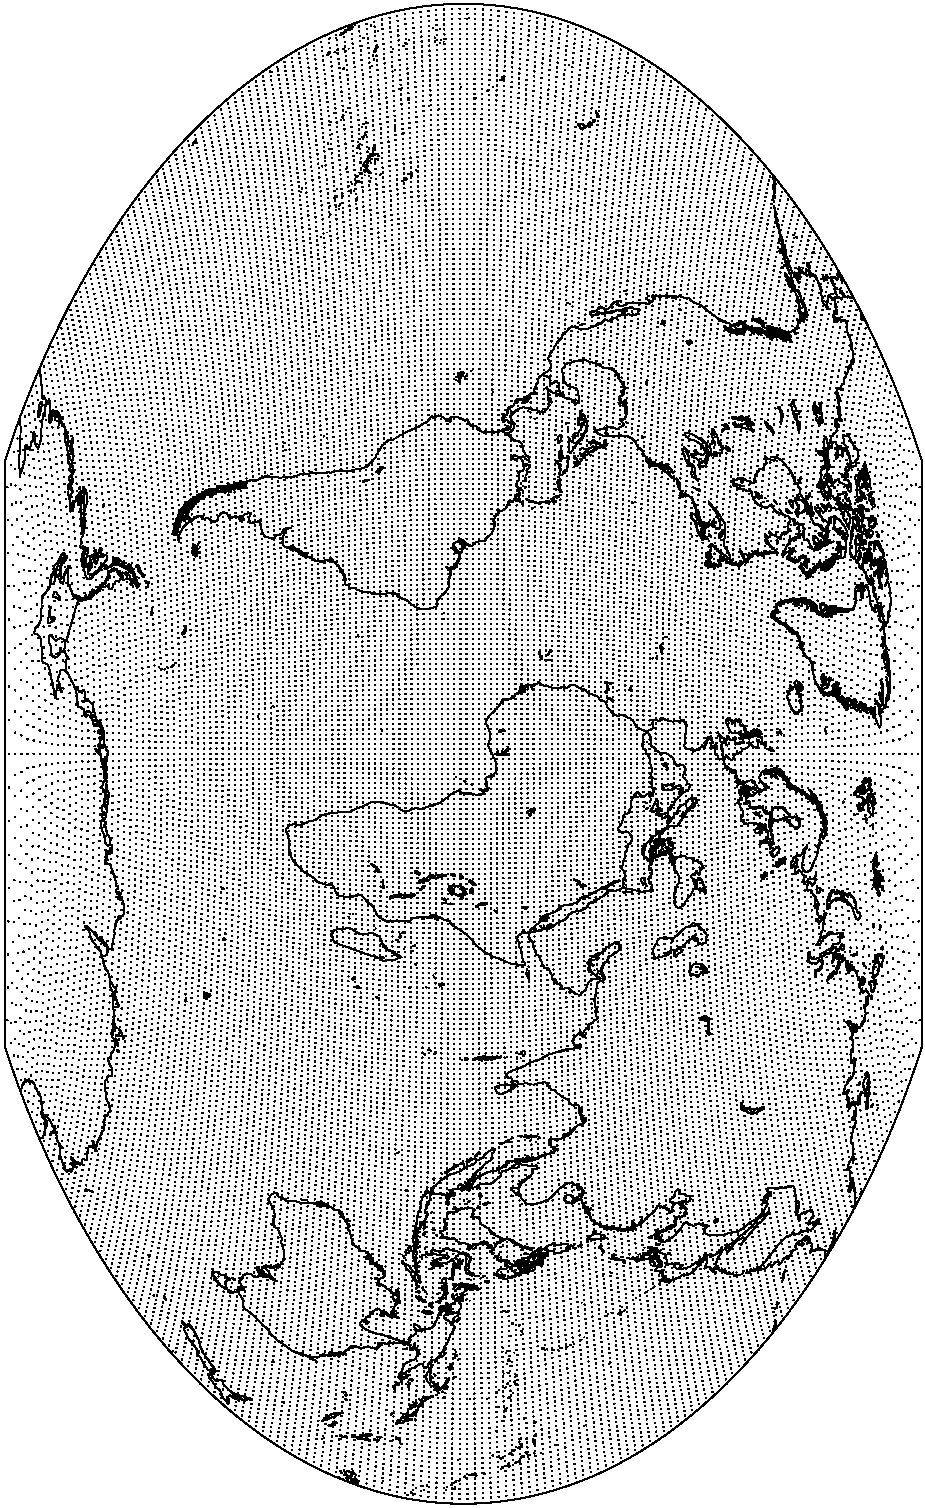
\includegraphics[height=0.75\linewidth,angle=90]{arp_6B60_grid0.pdf}
\captionof{figure}{Black dots: ARPEGE grid at truncation TL149 (set $\mathcal{S}^c_0$)}
\end{center}
\begin{center}
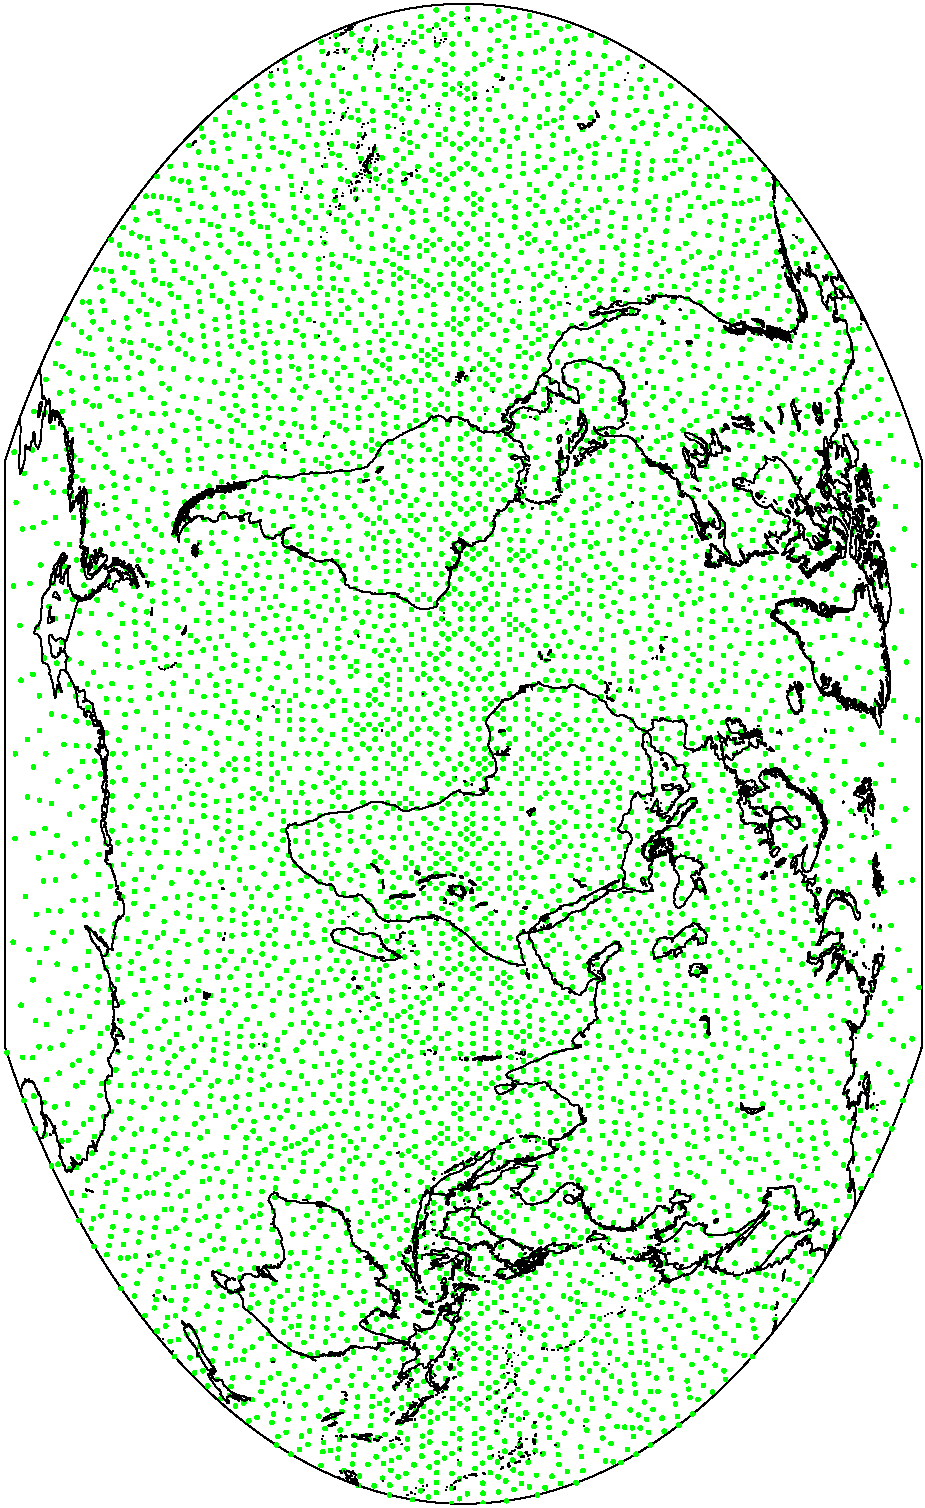
\includegraphics[height=0.75\linewidth,angle=90]{arp_6B60_grid1.pdf}
\captionof{figure}{Green dots: subset $\mathcal{S}^c_1$ for a homogeneous support radius $r^h$}
\end{center}

The vertical subsampling from $\mathcal{S}^l_0$ to $\mathcal{S}^l_1$ is defined similarly. At each horizontal point, we define the minimum vertical support radius over the whole level $i^l$:
\begin{align}
r^v_\mathrm{min}(i^l) = \min_{i^c \in \mathcal{S}^c_1} r^v(i^c,i^l)
\end{align}
The normalized distance between two levels $i^l$ and $j^l$ is defined as
\begin{align}
\widehat{d}^v_\text{min}(i^l,j^l) = \frac{d^v(i^l,j^l)}{\displaystyle \sqrt{\frac{1}{2}\left(\left(r^v_\mathrm{min}(i^l)\right)^2+\left(r^v_\mathrm{min}(j^l)\right)^2\right)}}
\end{align}
where $d^v(i^l,j^l)$ is the vertical distance between levels $i^l$ and $j^l$ (measured in meters or in pressure logarithm for instance). We start from the first level (always in the $\mathcal{S}^l_1$ subset) and look for the next vertical level for which the vertical normalized distance $\widehat{d}^v_\text{min}$ with the first level is larger than $1/\rho$. Thus, the distance $d^v$ between these levels is approximately $r^v/\rho$. Once such a level is reached, the procedure starts again towards the next one. The last level is automatically included in the $\mathcal{S}^l_1$ subset.

\begin{center}
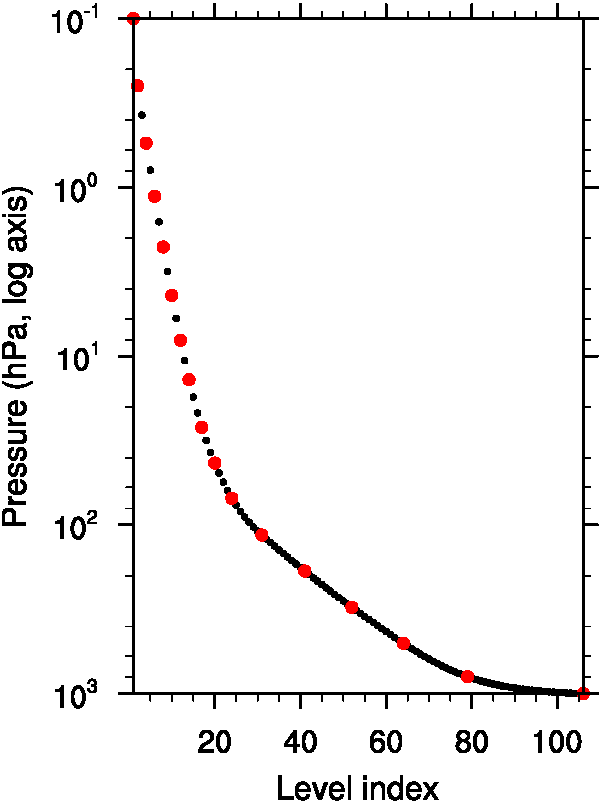
\includegraphics[height=0.6\linewidth]{profile.pdf}
\captionof{figure}{Black dots: ARPEGE levels; red dots: subset $\mathcal{S}^l_1$ with a homogeneous vertical support radius $r^v$ in pressure logarithm coordinate}
\end{center}

A final horizontal subsampling is applied for each level of $\mathcal{S}^l_1$ from $\mathcal{S}^c_1$ to $\mathcal{S}^c_2$. The trial-and-error algorithm select $n^c_2(i^l)$ horizontal points at each level $i^l \in \mathcal{S}^l_1$ with
\begin{align}
n^c_2(i^l) = \frac{2 \mathcal{A} \rho^2}{\sqrt{3} \left(\overbar{r^h}(i^l)\right)^2}
\end{align}
where
\begin{align}
\overbar{r^h}(i^l) = \frac{1}{n^c_1} \sum_{i^c \in \mathcal{S}^c_1} r^h(i^c,i^l)
\end{align}
is the horizontal average of $r^h$ at level $i^l$. The algorithm tries to maximize a normalized horizontal distance, defined between points $i^c$ and $j^c$ at level $i^l$ as
\begin{align}
\widehat{d}^s(i^c,j^c) = \frac{d^h(i^c,j^c)}{\displaystyle \sqrt{\frac{1}{2}\left(\left(r^h(i^c,i^l)\right)^2+\left(r^h(j^c,i^l)\right)^2\right)}}
\end{align}

\begin{center}
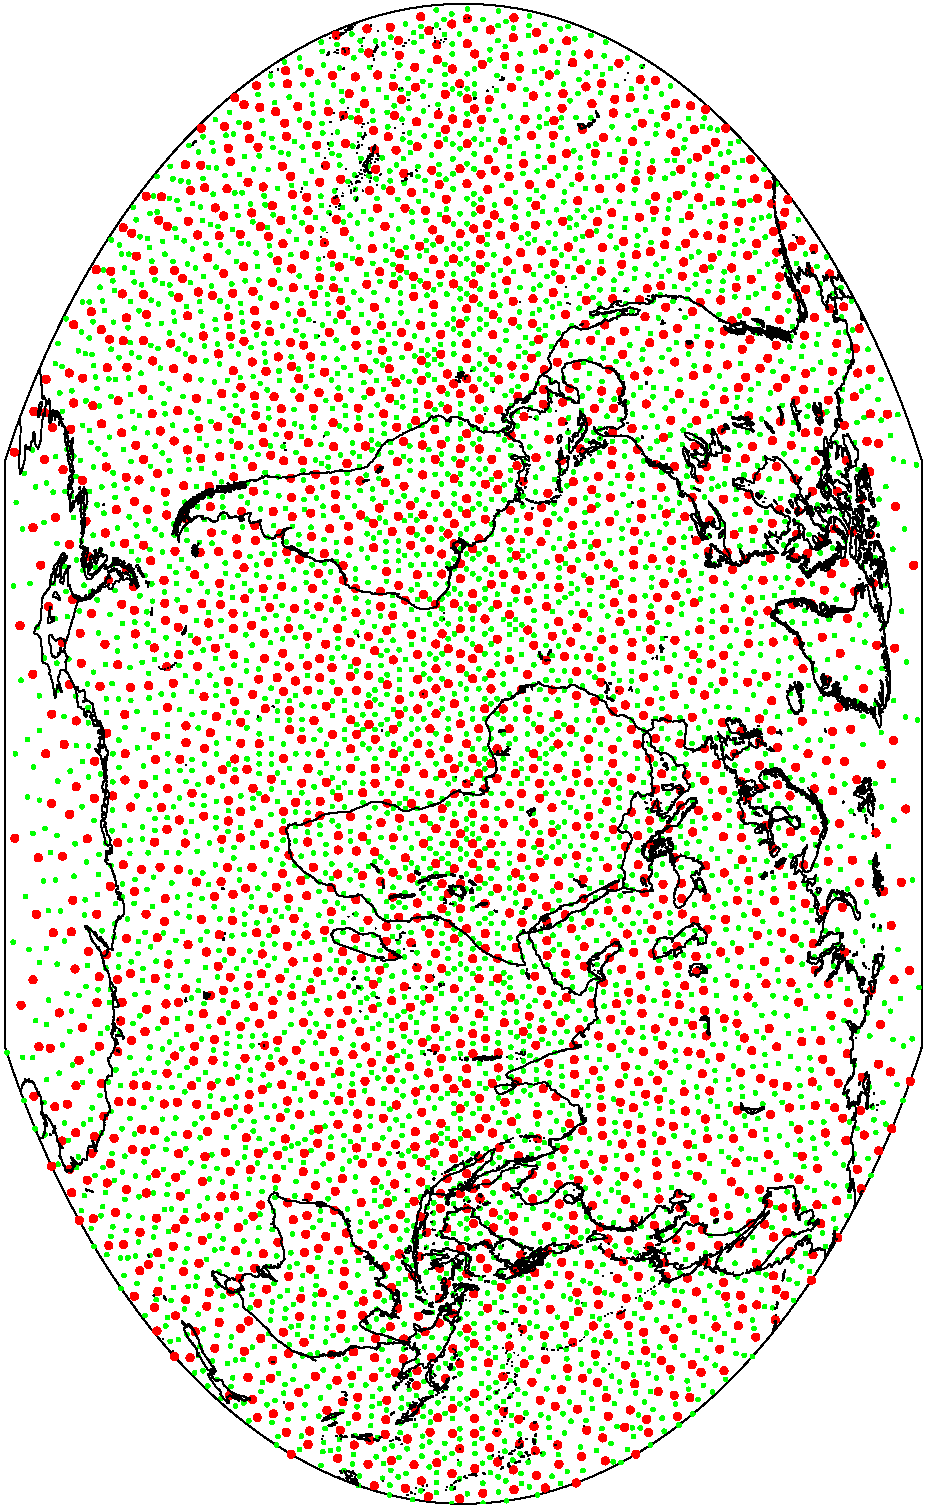
\includegraphics[height=0.65\linewidth,angle=90]{arp_6B60_grid2_12.pdf}
\captionof{figure}{Red dots: subset $\mathcal{S}^c_2$ at a level with a small support radius $r^h$}
\end{center}
\begin{center}
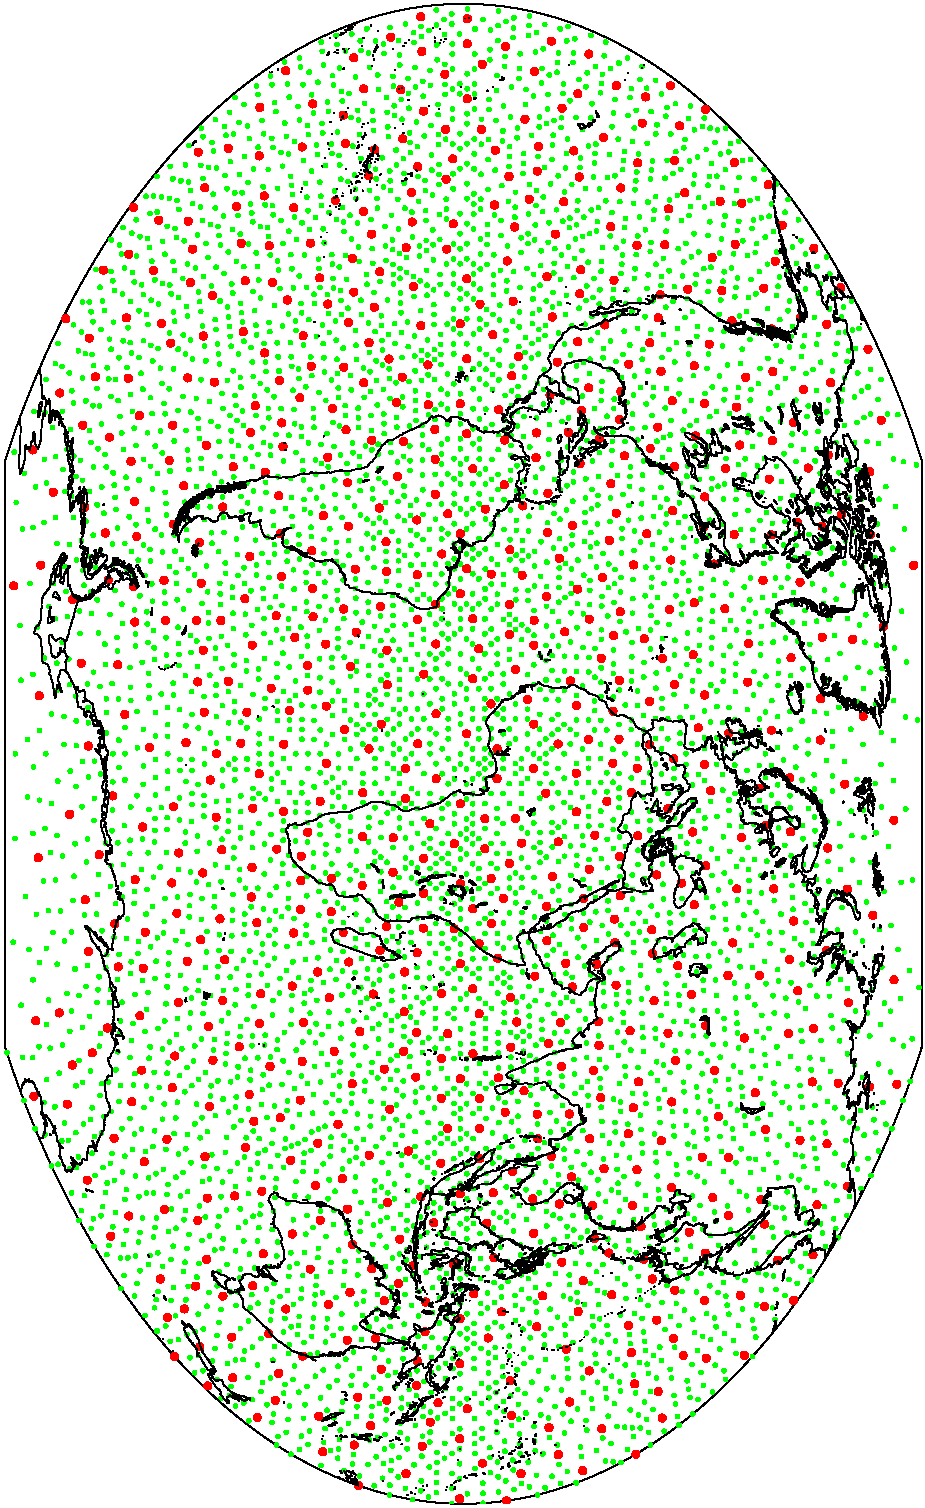
\includegraphics[height=0.65\linewidth,angle=90]{arp_6B60_grid2_8.pdf}
\captionof{figure}{Red dots: subset $\mathcal{S}^c_2$ at a level with a moderate support radius $r^h$}
\end{center}
\begin{center}
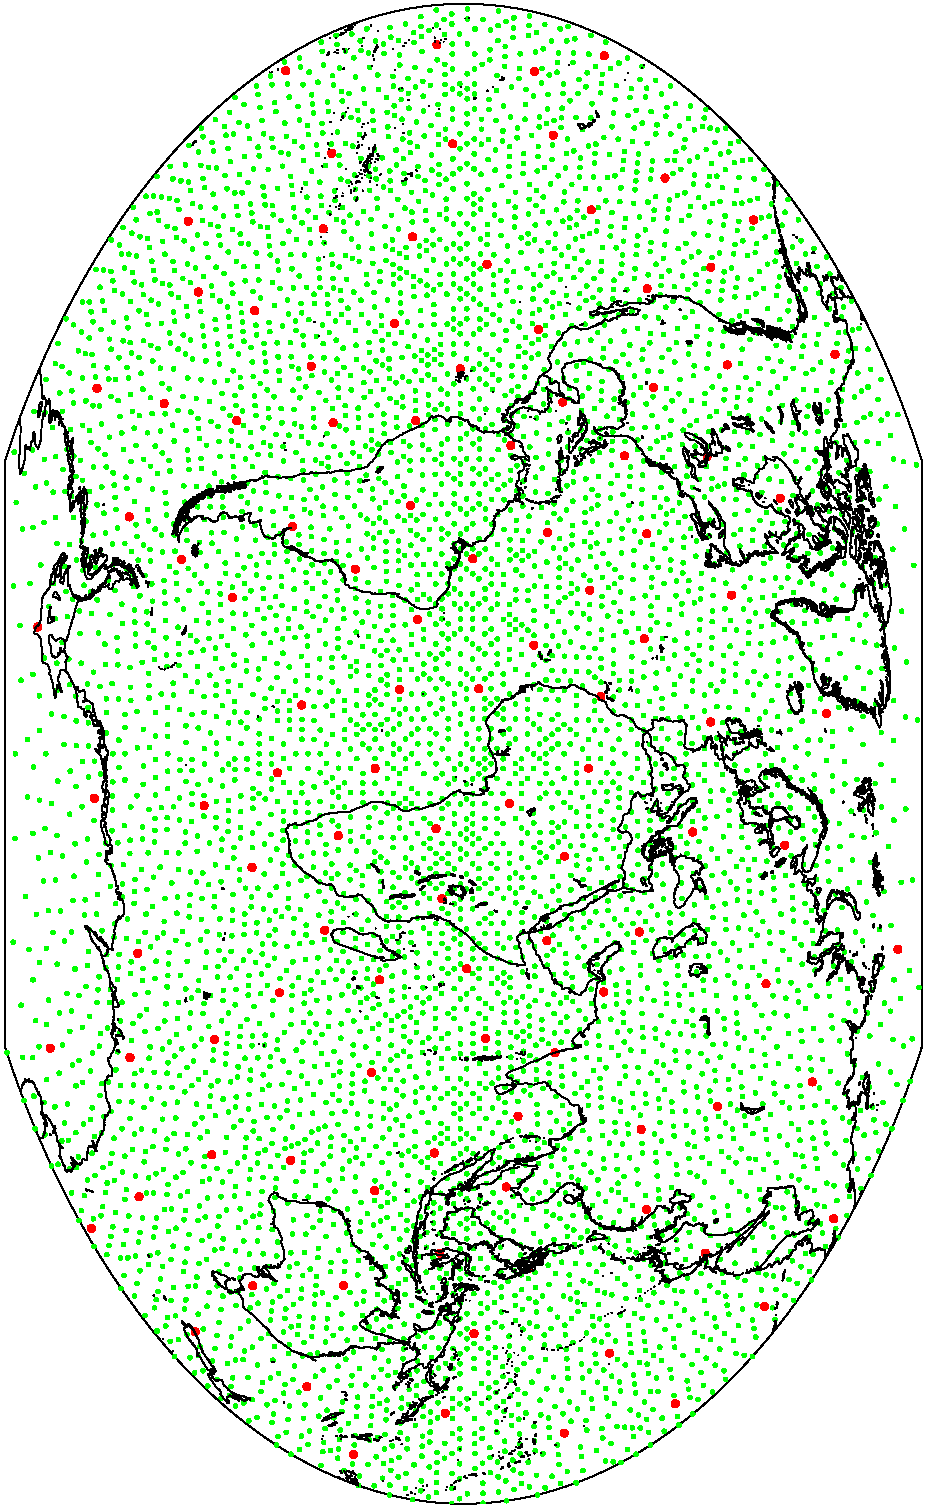
\includegraphics[height=0.65\linewidth,angle=90]{arp_6B60_grid2_2.pdf}
\captionof{figure}{Red dots: subset $\mathcal{S}^c_2$ at a level with a large support radius $r^h$}
\end{center}

The trial-and-error algorithm is able to detect the local variations of support radius $r^h$ to adapt the subgrid, as shown by Figures \ref{fig:mesh_homogeneous} and \ref{fig:mesh_heterogeneous}. The larger the support radius $r^h$, the coarser the subgrid mesh.

\begin{center}
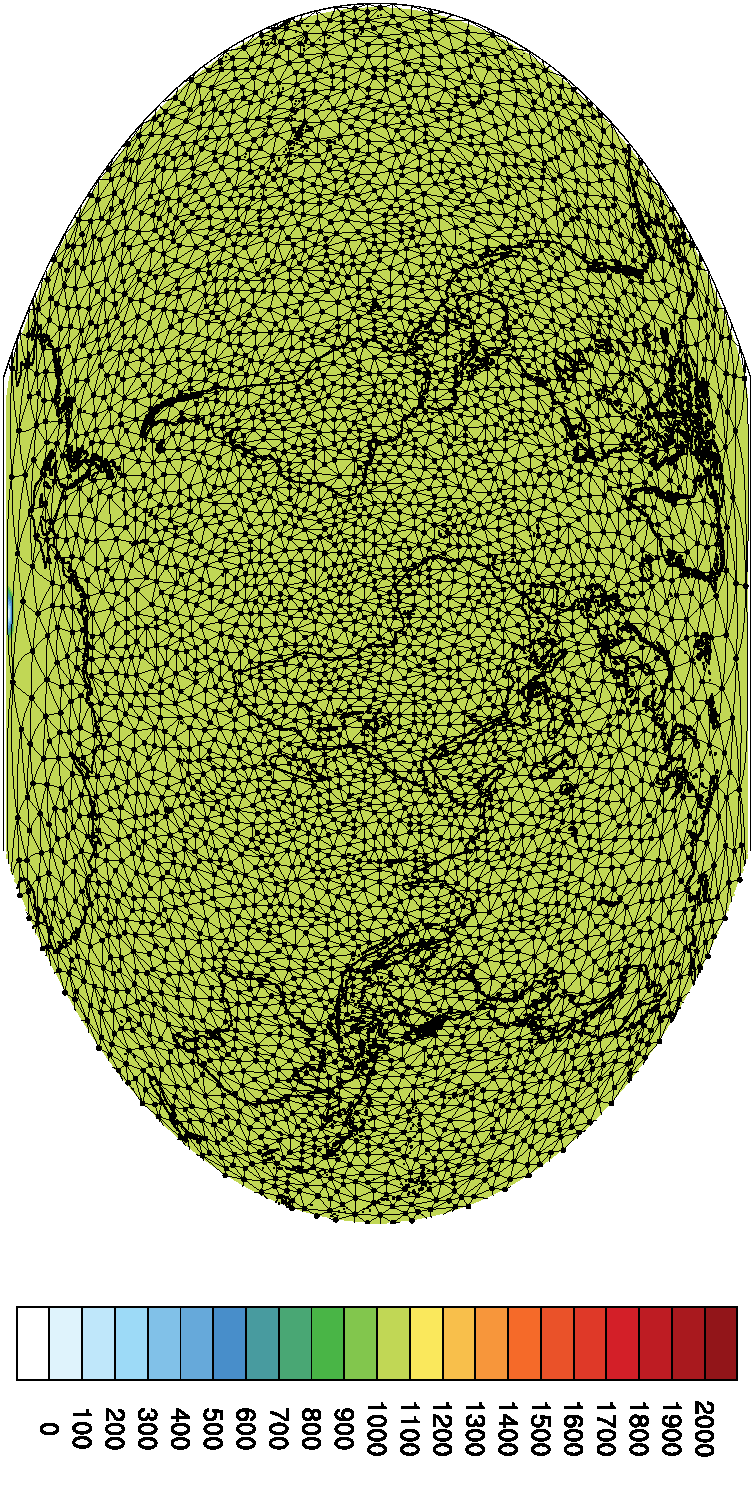
\includegraphics[height=0.9\linewidth,angle=90]{arp_6B60_mesh_001_homogeneous.pdf}
\captionof{figure}{Subset $\mathcal{S}^c_2$ for a homogeneous support radius $r^h$ \label{fig:mesh_homogeneous}}
\end{center}
\begin{center}
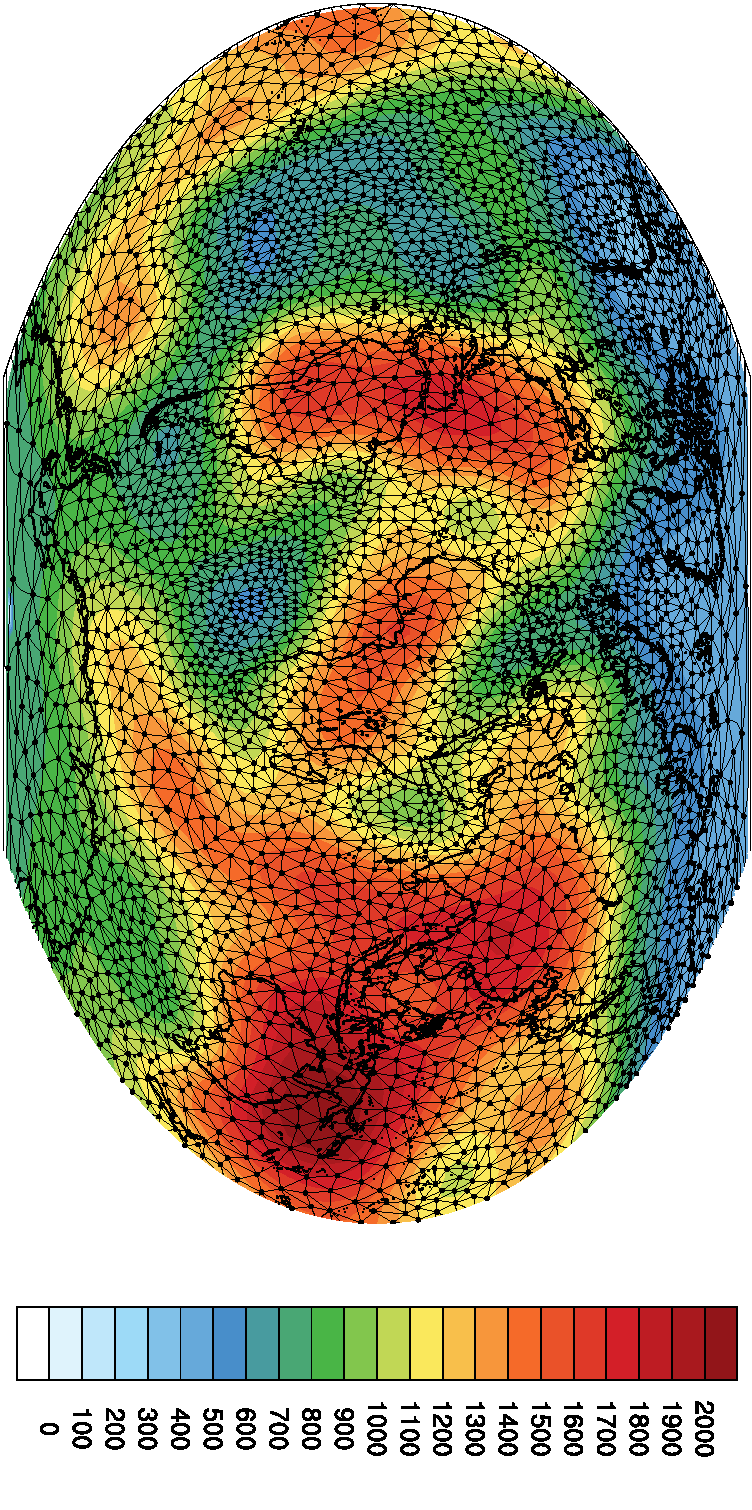
\includegraphics[height=0.9\linewidth,angle=90]{arp_6B60_mesh_001_heterogeneous.pdf}
\captionof{figure}{Subset $\mathcal{S}^c_2$ for a smoothly heterogeneous support radius $r^h$ \label{fig:mesh_heterogeneous}}
\end{center}

\section{Convolution function}

\subsection{Distance-based approach}
The convolution function used in NICAS is the famous \citet{gaspari_1999} function (GC99 hereafter), adapted to a the case where the distance is normalized by the support radius:
\begin{align}
\mathcal{C}(\widehat{d}) = \left\{
\begin{array}{ll}
\displaystyle
1 - 8 \widehat{d}^5 + 8 \widehat{d}^4 + 5 \widehat{d}^3 - \frac{20}{3} \widehat{d}^2 & \displaystyle \text{if }\widehat{d} \le \frac{1}{2} \\[2ex]
\displaystyle
\frac{8}{3} \widehat{d}^5 - 8 \widehat{d}^4 + 5 \widehat{d}^3 + \frac{20}{3} \widehat{d}^2 - 10 \widehat{d} + 4 - \frac{1}{3} \widehat{d}^{-1} & \displaystyle \text{if }\frac{1}{2} < \widehat{d} \le 1 \\[2ex]
\displaystyle
0 & \text{if } 1 < \widehat{d}
\end{array} \right.
\end{align}
where $\widehat{d}$ is a normalized distance (great-circle distance divided by the compact support radius).\\
$  $\\
The 3D normalized distance between nodes with coordinates $(i^c,i^l)$ and $(j^c,j^l)$ is:
\begin{align}
\widehat{d}(i^c,i^l;j^c,j^l) = \sqrt{\left(\widehat{d}^h(i^c,i^l;j^c,j^l)\right)^2+\left(\widehat{d}^v(i^c,i^l;j^c,j^l)\right)^2}
\end{align}
where $\widehat{d}^h$ and $\widehat{d}^v$ are the horizontal and vertical normalized distances, respectively given by:
\begin{align}
\widehat{d}^h(i^c,i^l;j^c,j^l) = \frac{d^h(i^c,j^c)}{\displaystyle \sqrt{\frac{1}{2}\left(\left(r^h(i^c,i^l)\right)^2+\left(r^h(j^c,j^l)\right)^2\right)}}
\end{align}
\begin{align}
\widehat{d}^v(i^c,i^l;j^c,j^l) = \frac{d^v(i^l,j^l)}{\displaystyle \sqrt{\frac{1}{2}\left(\left(r^v(i^c,i^l)\right)^2+\left(r^v(j^c,j^l)\right)^2\right)}}
\end{align}

This approach is valid for homogeneous and smoothly varying support radii, whose variations length-scale is larger than the convolution function length-scale, as shown by Figures \ref{fig:diracs_homogeneous} and \ref{fig:diracs_heterogeneous}.

\begin{center}
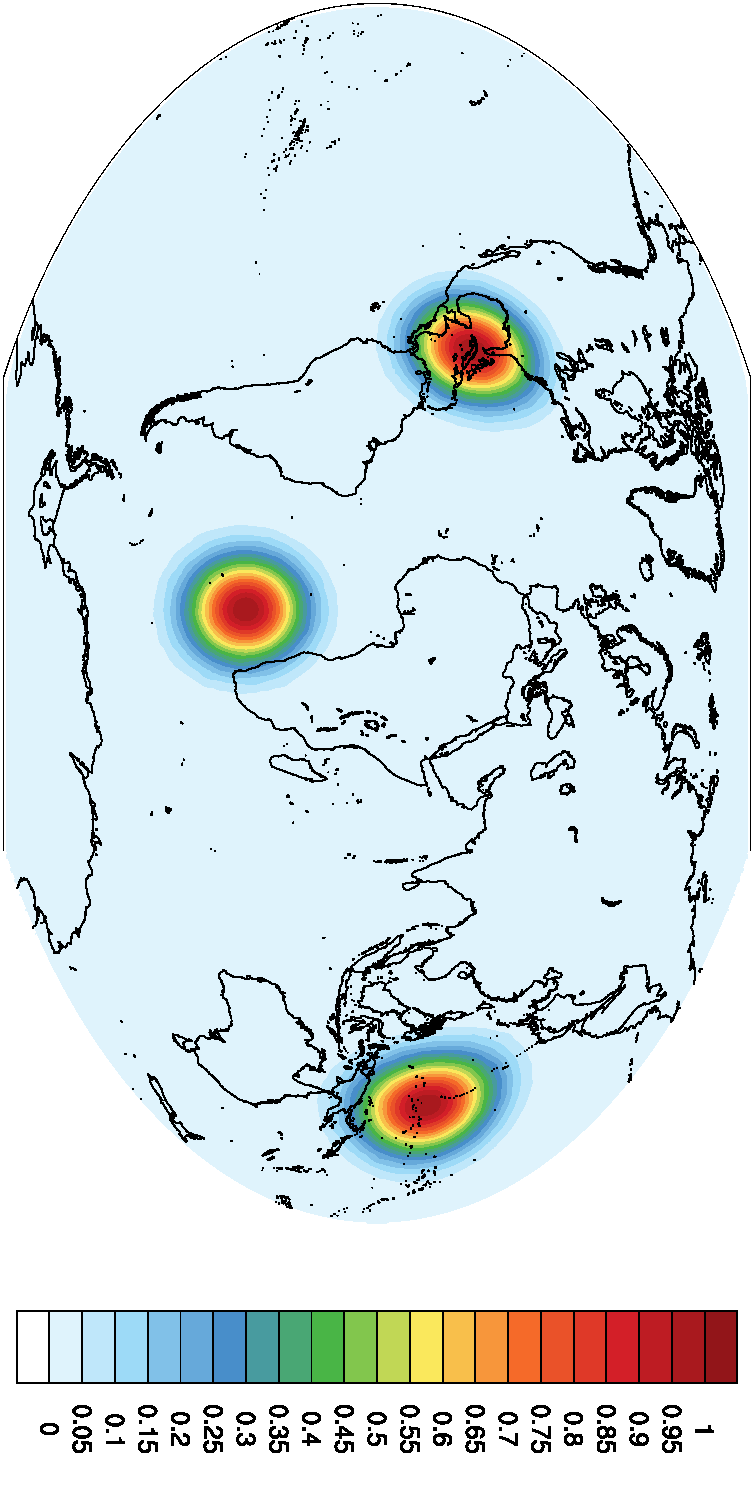
\includegraphics[height=0.85\linewidth,angle=90]{arp_6B60_dirac_001_homogeneous.pdf}
\captionof{figure}{Convolution functions for a homogeneous support radius $r^h$ \label{fig:diracs_homogeneous}}
\end{center}
\begin{center}
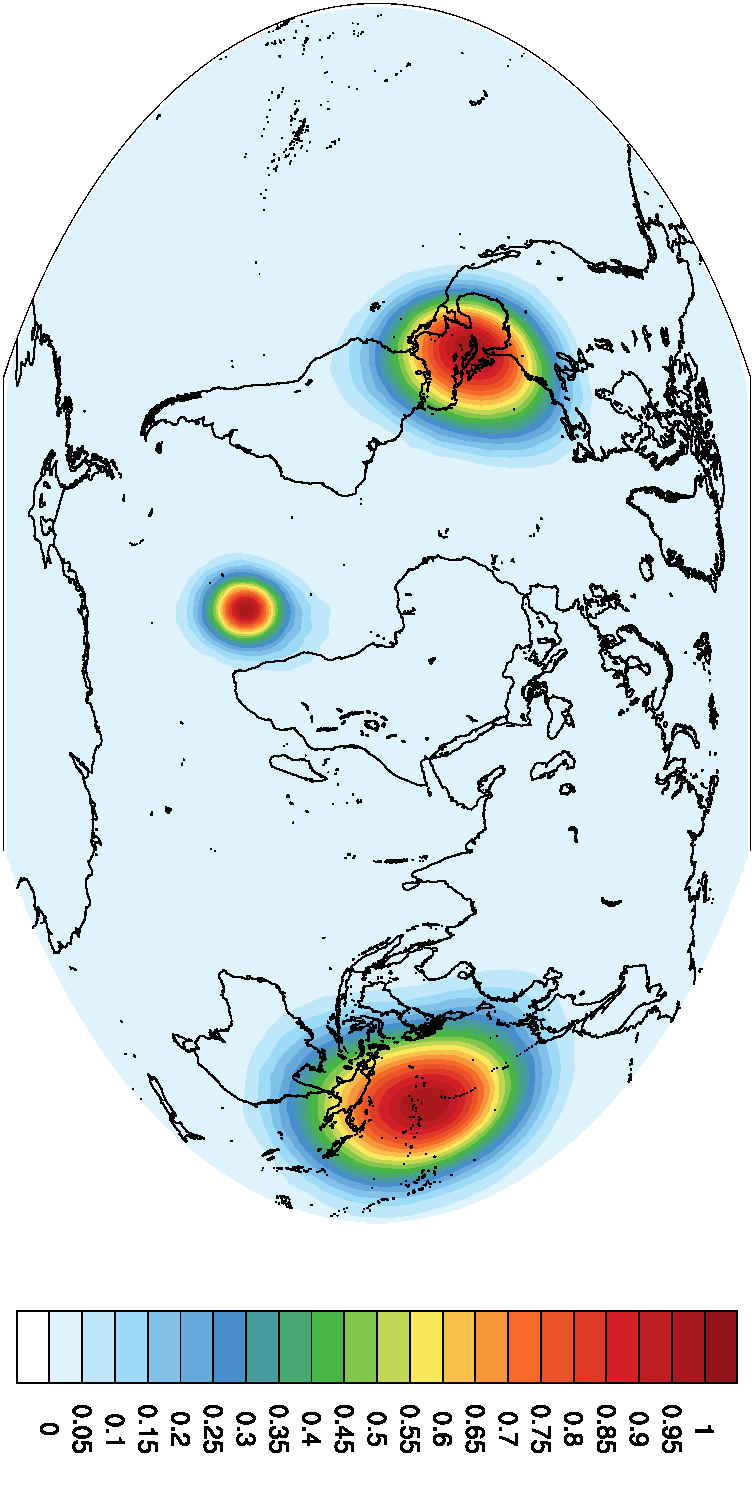
\includegraphics[height=0.85\linewidth,angle=90]{arp_6B60_dirac_001_heterogeneous.pdf}
\captionof{figure}{Convolution functions for a smoothly heterogeneous support radius $r^h$ \label{fig:diracs_heterogeneous}}
\end{center}

\subsection{Network-based approach}
If $r^h$ and $r^v$ are heterogeneous and rapidly varying, the distance-based approach is irrelevant. Figures \ref{fig:mesh_distance_network} and \ref{fig:dirac_distance} show a case with a belt of lower support radius $r^h$ is surrounding the point where the convolution function is applied. Since the values of the convolution function depends on the support radii at the center and at the concerned nodes only, the function values outside this lower radius belt are not affected by it. This is an issue: the signal should be less propagated through a zone a lower radius $r^h$.

\begin{center}
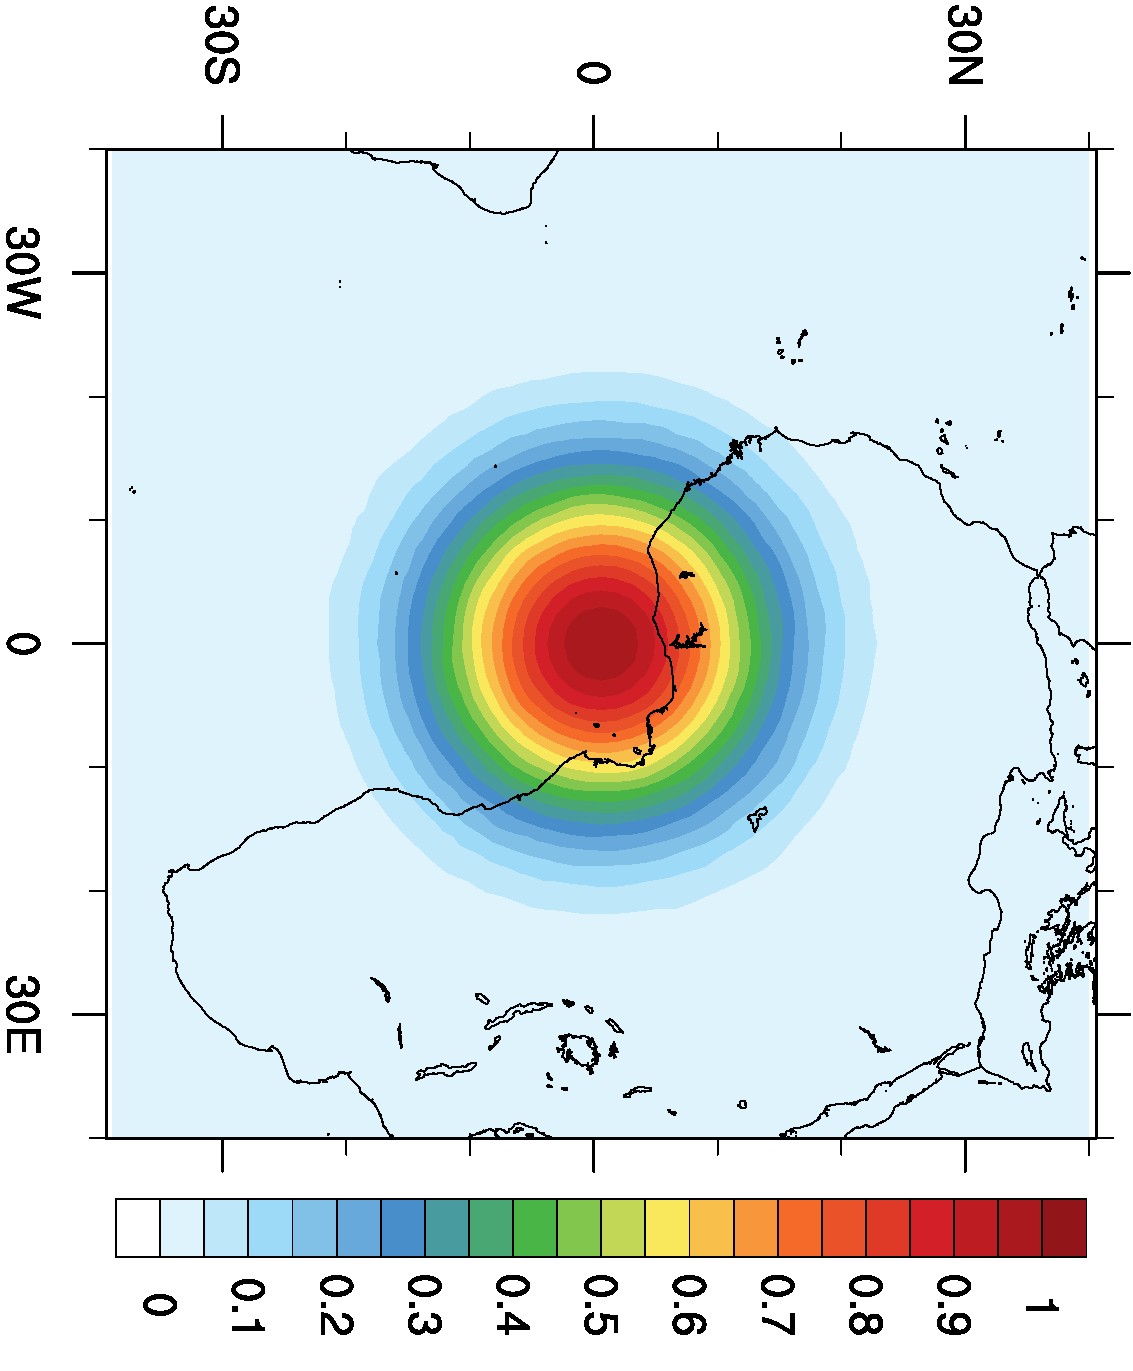
\includegraphics[height=0.63\linewidth,angle=90]{arp_6B60_dirac_001_ref.pdf}
\captionof{figure}{Convolution function for a homogeneous support radius $r^h$ \label{fig:dirac_homogeneous}}
\end{center}
\begin{center}
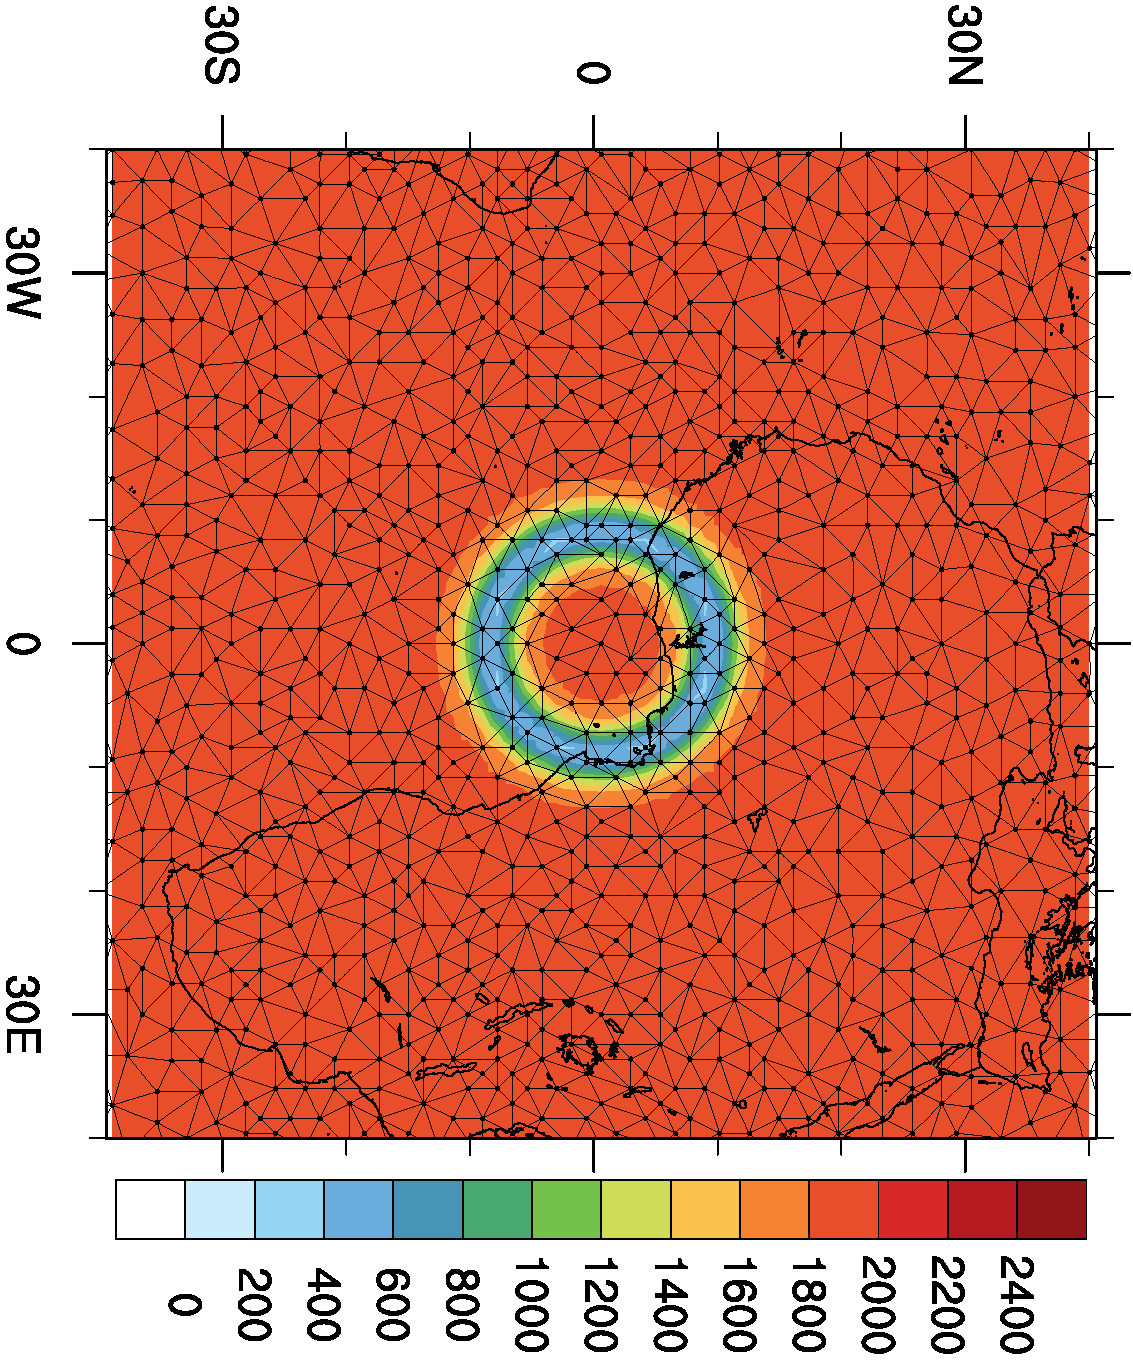
\includegraphics[height=0.63\linewidth,angle=90]{arp_6B60_mesh_001_distance_network.pdf}
\captionof{figure}{Heterogeneous support radius $r^h$ and subset $\mathcal{S}^c_2$ (black dots) \label{fig:mesh_distance_network}}
\end{center}
\begin{center}
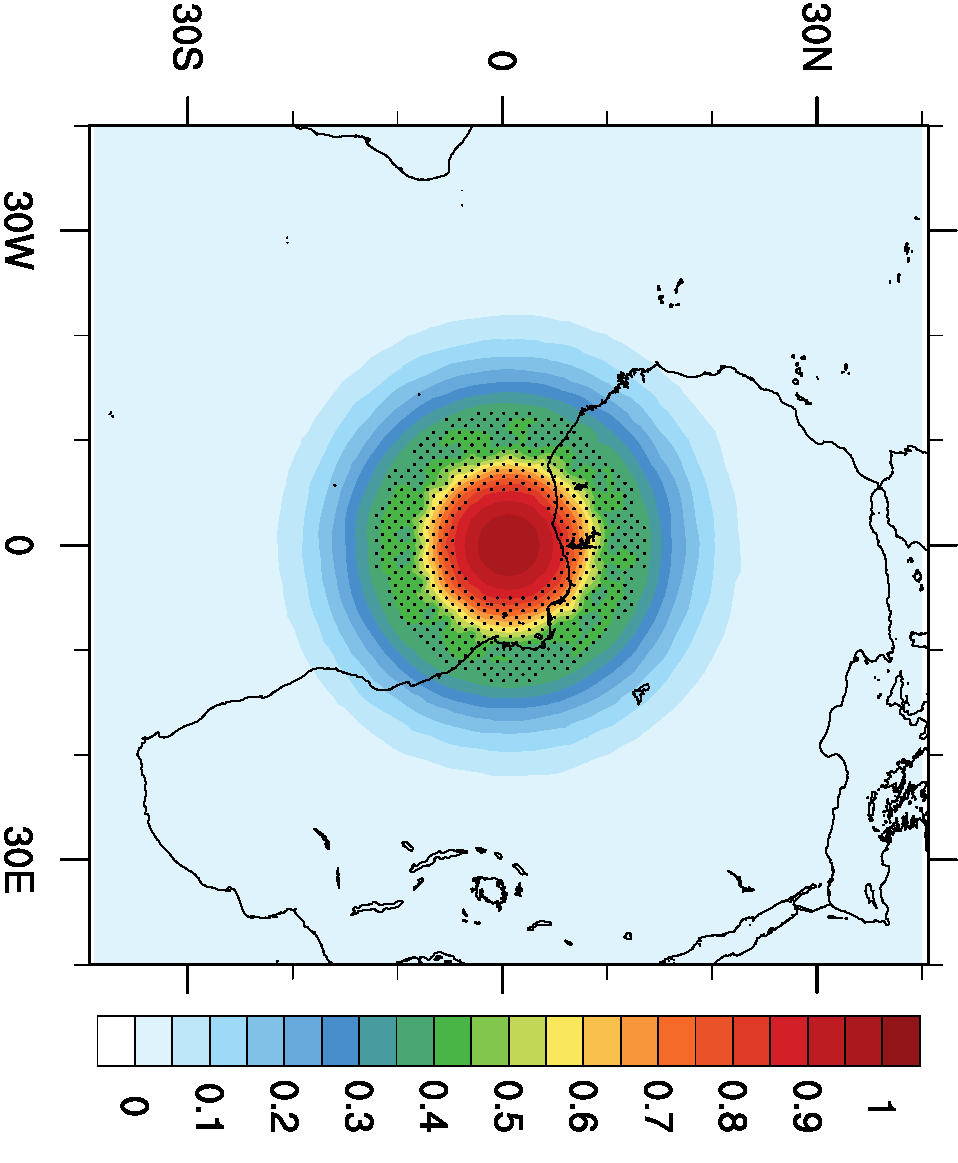
\includegraphics[height=0.63\linewidth,angle=90]{arp_6B60_dirac_001_distance.pdf}
\captionof{figure}{Convolution function for a heterogeneous support radius $r^h$ with the distance-based approach; zone of lower $r^h$ (dotted) \label{fig:dirac_distance}}
\end{center}

A simple solution is to switch to a network-based approach. First, we compute all the 3D normalized distances between nearest neighbors on the full grid $\mathcal{G}^f$. Then, the normalized distance between to non-neighbor nodes is computed as the shortest integrated normalized distance on a path along $\mathcal{G}^f$ nodes. Figure \ref{fig:dirac_network} shows that this method is able to provide the expected result: the signal is less propagated through the belt of lower radius $r^h$. All the nodes within and beyond that belt are affected.

\begin{center}
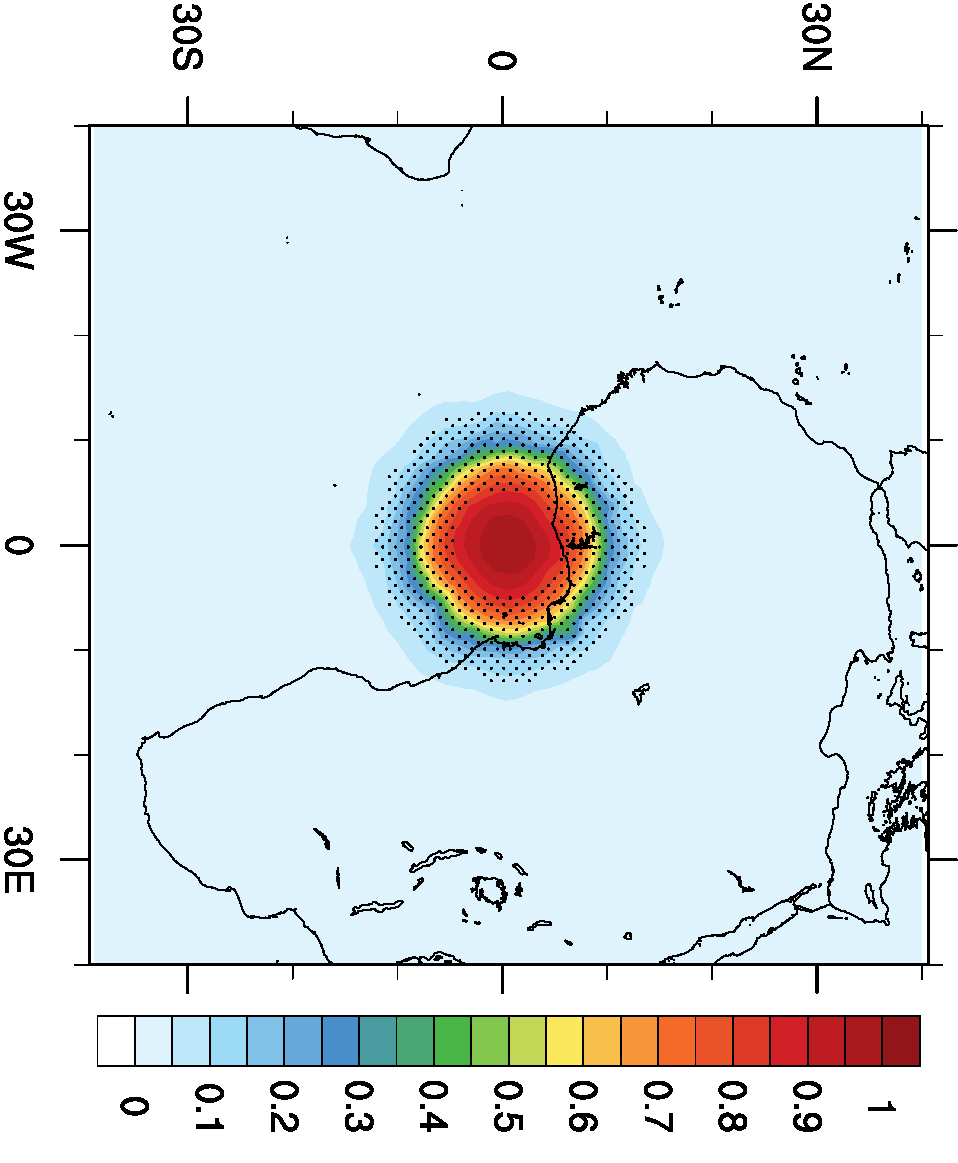
\includegraphics[height=0.63\linewidth,angle=90]{arp_6B60_dirac_001_network.pdf}
\captionof{figure}{Convolution function for a heterogeneous support radius $r^h$ with the network-based approach; zone of lower $r^h$ (dotted) \label{fig:dirac_network}}
\end{center}

This network-based approach can deal with complex boundaries in a better way than the distance-based approach, for which complex boundaries are just a mask applied on the underlying convolution functions. Figure \ref{fig:nemo_dirac} shows for the NEMO grid that the network-based approach is able to contain the convolution function to the West side of the Isthmus of Panama (interpolation has to be adapted so that bilinear interpolation triangles do not cross mask boundaries). This approach can also limit the signal propagation from the West coast to the East coast of Florida. However, it is not a full integrative method as diffusion-based methods. For instance, the width of straits is not taken into account to propagate the signal, only the distance around obstacles matters.

\begin{center}
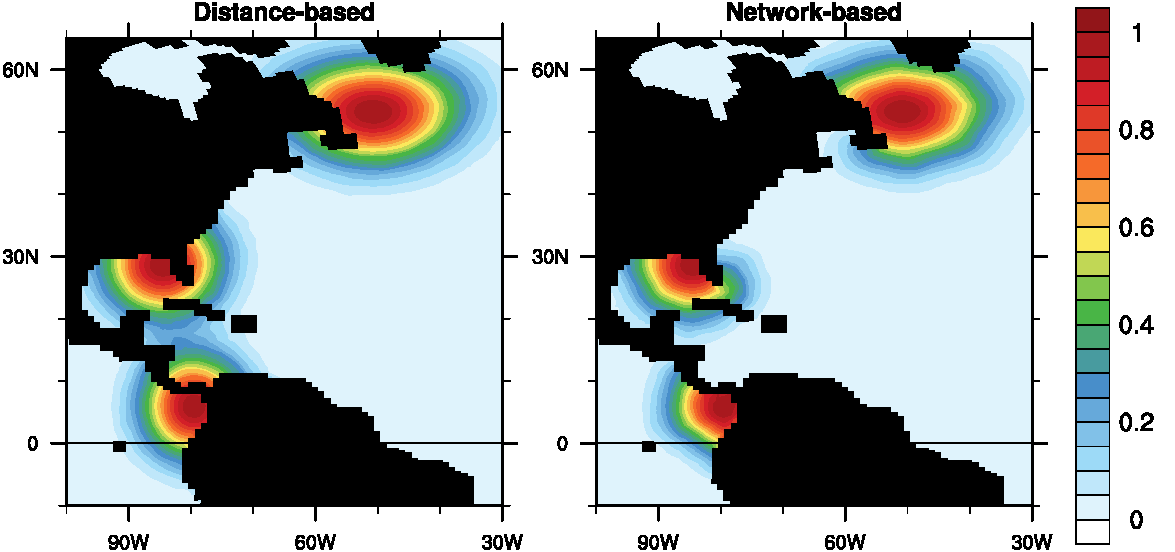
\includegraphics[width=0.9\linewidth]{nemo_dirac_001.pdf}
\captionof{figure}{Convolution functions with complex boundaries of the NEMO grid, for a distance-based approach (left) and a network-based approach (right) \label{fig:nemo_dirac}}
\end{center}

\section{Normalization}
As mentioned in the introduction, even if the subgrid convolution matrix $\mathbf{C}^s$ is normalized, $\mathbf{S} \mathbf{C}^s \mathbf{S}^\mathrm{T}$ is not normalized everywhere (only on the nodes of $\mathcal{G}^s$). As a consequence, a normalization operator $\mathbf{N}$ (diagonal) is applied on both sides of $\mathbf{S} \mathbf{C}^s \mathbf{S}^\mathrm{T}$, to ensure that $\widetilde{\mathbf{C}}$ is exactly normalized.\\
$  $\\
The simpler method to compute $\mathbf{N}$ would be to apply $\mathbf{S} \mathbf{C}^s \mathbf{S}^\mathrm{T}$ to a Dirac vector $\boldsymbol{\delta}_i$:
\begin{align}
N_{ii} = \left(\boldsymbol{\delta}_i^\mathrm{T} \mathbf{S} \mathbf{C}^s \mathbf{S}^\mathrm{T} \boldsymbol{\delta}_i\right)^{-1/2}
\end{align}
where $\boldsymbol{\delta}_i \in \mathbb{R}^n$ is a vector of zeros with only the $i^\text{th}$ coefficient equal to one. However, the cost of applying the full $\mathbf{S} \mathbf{C}^s \mathbf{S}^\mathrm{T}$ to Dirac vectors at each node of the full grid $\mathcal{G}^f$ is prohibitive.\\
$  $\\
If we look at the details of the previous operations though, the number of relevant nodes involved in the computation of $N_{ii}$ is very limited:
\begin{itemize}
\item 1 node of $\mathcal{G}^f$ is non-zero in $\boldsymbol{\delta}_i$,
\item up to 3 nodes of $\mathcal{G}^h$ are non-zero in $\mathbf{S}^{h\textrm{T}} \boldsymbol{\delta}_i$ (bilinear interpolation),
\item up to 6 nodes of $\mathcal{G}^v$ are non-zero in $\mathbf{S}^{v\textrm{T}} \mathbf{S}^{h\textrm{T}} \boldsymbol{\delta}_i$ (linear interpolation),
\item up to 18 nodes of $\mathcal{G}^s$ are non-zero in $\mathbf{S}^{s\textrm{T}} \mathbf{S}^{v\textrm{T}} \mathbf{S}^{h\textrm{T}} \boldsymbol{\delta}_i$ (bilinear interpolation),
\end{itemize}
Thus, the convolution of these 18 non-zero nodes only has an impact on $N_{ii}$. An affordable procedure is the following:
\begin{enumerate}
\item computing the 18 non-zero values of $\mathbf{S}^{s\textrm{T}} \mathbf{S}^{v\textrm{T}} \mathbf{S}^{h\textrm{T}} \boldsymbol{\delta}_i$ and storing them in a vector $\boldsymbol{\delta}' \in \mathbb{R}^{18}$,
\item applying the relevant block of the subgrid convolution matrix $\mathbf{C}^s$ to the coefficients of $\boldsymbol{\delta}'$ and storing only the result for these coefficients in a vector $\boldsymbol{\delta}'' \in \mathbb{R}^{18}$,
\item computing the final result as the inverse square-root of a scalar product: $N_{ii} = \left\langle \boldsymbol{\delta}',\boldsymbol{\delta}''\right\rangle^{-1/2}$.
\end{enumerate}
The computational cost of this procedure is far lower than applying the full $\mathbf{S} \mathbf{C}^s \mathbf{S}^\mathrm{T}$. Besides, the procedure can be applied in parallel to all nodes, dividing the elapsed time by the number of parallel threads.\\
$  $\\
This normalization procedure does not rely on an explicit formula that would be derived in a continuous framework. Thus, it is exact for both homogeneous and heterogeneous support radii, and also in the presence of complex boundaries.

\section{Square-root formulation}

\subsection{Approximate solution}
Data assimilation solvers often require a square-root $\mathbf{U}$ of the localization matrix $\mathbf{C}$, such that $\mathbf{C} = \mathbf{U} \mathbf{U}^\textrm{T}$. For the NICAS method:
\begin{align}
\widetilde{\mathbf{U}} = \mathbf{N} \mathbf{S} \mathbf{U}^s
\end{align}
is a square-root of $\widetilde{\mathbf{C}}$ if $\mathbf{U}^s$ is a square-root of $\mathbf{C}^s$. However, computing an exact square-root of $\mathbf{C}^s$ is not affordable with explicit methods (ex. Cholesky decomposition) if $n^s$ is too large. An approximate square-root can be obtained by noting that:
\begin{itemize}
\item the (convolution) square-root of a Gaussian function with a homogeneous length-scale $L$ is also a Gaussian function with a homogeneous length-scale $L/\sqrt{2}$,
\item the GC99 function has a Gaussian-like shape.
\end{itemize}
Thus, an approximate square-root of $\mathbf{C}^s$ can be modeled as follows:
\begin{align}
\mathbf{U}^s = \mathbf{N}' \mathbf{V}^s
\end{align}
where:
\begin{itemize}
\item $\mathbf{V}^s \in \mathbb{R}^{n^s \times n^s}$ is convolution matrix on the same subgrid $\mathcal{G}^s$ as $\mathbf{C}^s$, but with support radii divided by $\sqrt{2}$,
\item $\mathbf{N}' \in \mathbb{R}^{n^s \times n^s}$ is a diagonal normalization matrix ensuring that $\mathbf{U}^s \mathbf{U}^{s^\mathrm{T}} = \mathbf{N}' \mathbf{V}^s \mathbf{V}^{s\mathrm{T}} \mathbf{N}^{\prime\textrm{T}}$ is exactly normalized (as $\mathbf{C}^s$ is).
\end{itemize}
Thus, an approximate square-root of $\widetilde{\mathbf{C}}$ is given by $\widetilde{\mathbf{U}} \in \mathbb{R}^{n \times n^s}$:
\begin{align}
\widetilde{\mathbf{U}} = \mathbf{N} \mathbf{S} \mathbf{N}' \mathbf{V}^s
\end{align}
The control vector state corresponding to this square-root has a size $n^s$, which is significantly smaller than $n$.\\
$  $\\
The difference between applying $\widetilde{\mathbf{C}}$ or $\widetilde{\mathbf{U}} \widetilde{\mathbf{U}}^\textrm{T}$ with $\widetilde{\mathbf{U}}$ being an approximate square-root is small, as shown by Figure \ref{fig:diracs_homogeneous_sqrt} (to be compared with Figure \ref{fig:diracs_homogeneous}) for a homogeneous support radius and Figure \ref{fig:mesh_heterogeneous_sqrt} (to be compared with Figure \ref{fig:mesh_heterogeneous}) for a heterogenous support radius.

\begin{center}
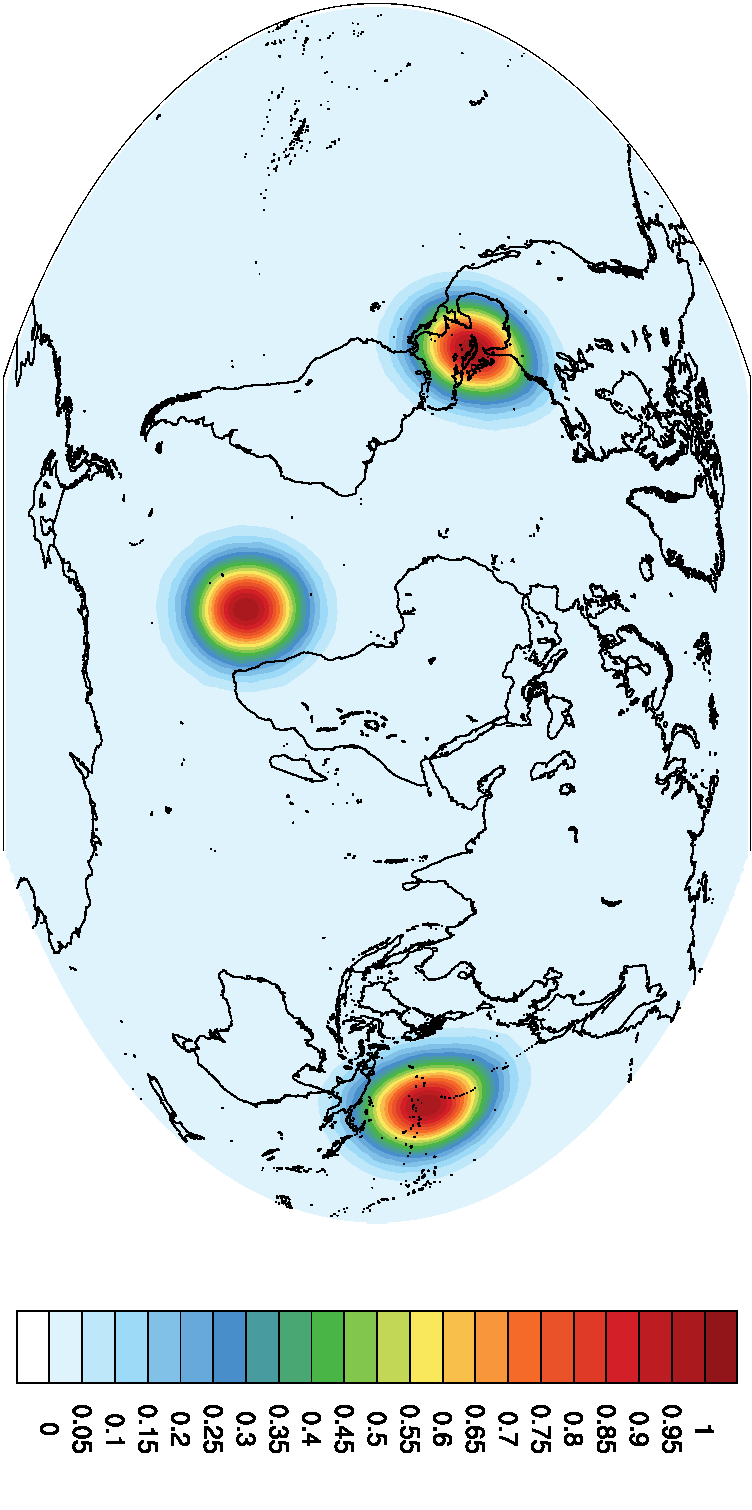
\includegraphics[height=0.88\linewidth,angle=90]{arp_6B60_dirac_001_homogeneous_sqrt.pdf}
\captionof{figure}{Convolution functions for a homogeneous support radius $r^h$, applied with the square-root formulation $\widetilde{\mathbf{U}} \widetilde{\mathbf{U}}^\textrm{T}$ \label{fig:diracs_homogeneous_sqrt}}
\end{center}
\begin{center}
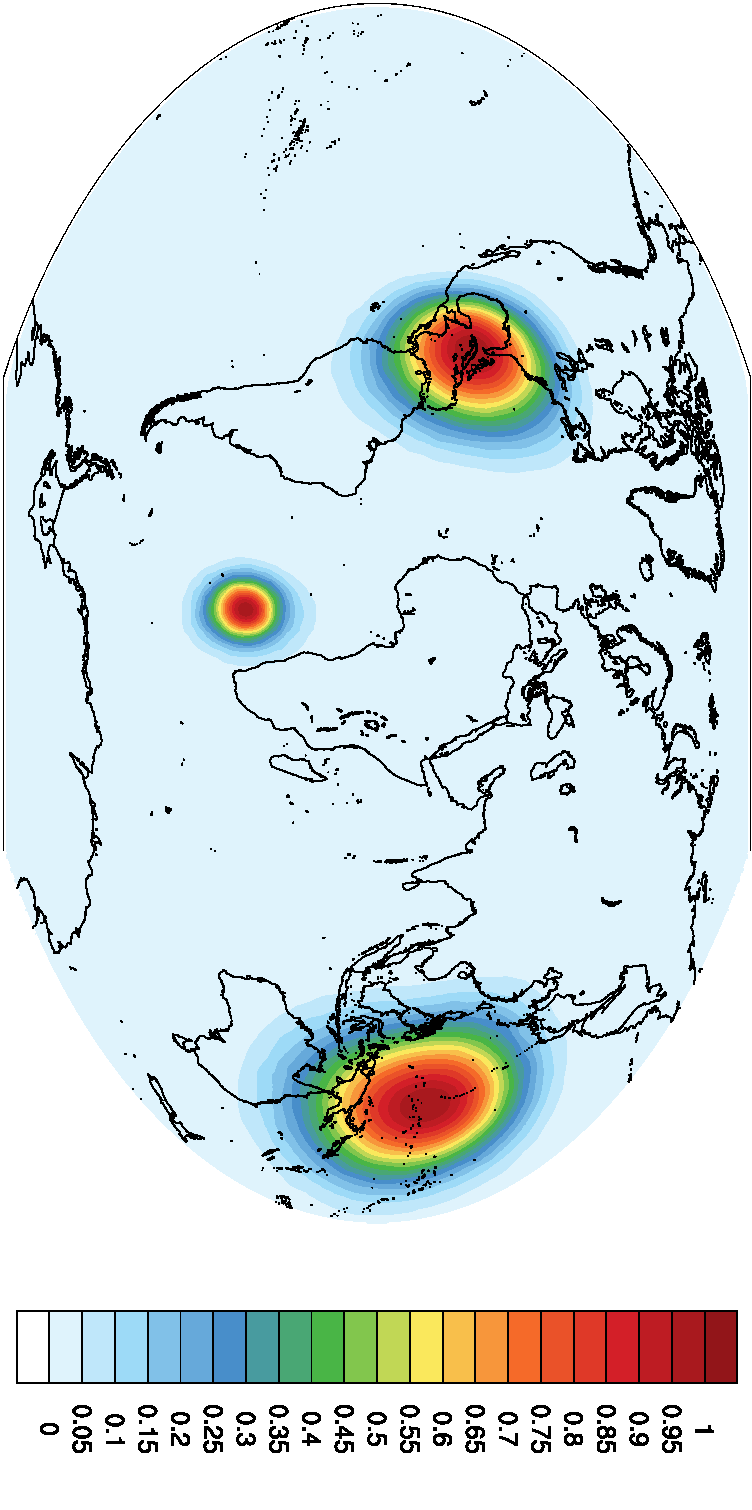
\includegraphics[height=0.88\linewidth,angle=90]{arp_6B60_dirac_001_heterogeneous_sqrt.pdf}
\captionof{figure}{Convolution functions for a smoothly heterogeneous support radius $r^h$, applied with the square-root formulation $\widetilde{\mathbf{U}} \widetilde{\mathbf{U}}^\textrm{T}$ \label{fig:mesh_heterogeneous_sqrt}}
\end{center}

\subsection{Impact on the normalization procedure}
Since the square-root defined in the previous section is only approximate, the normalization procedure has to be updated.\\
$  $\\
The first step is to compute the internal normalization $\mathbf{N}'$. The basic method is applied: for each node of the subgrid $\mathcal{G}^s$, the convolution adjoint $\mathbf{V}^{s\textrm{T}}$ is applied to a Dirac vector at the concerned node. Only the non-zero values inside the compact support of reduced size (divided by $\sqrt{2}$) are stored in a vector. The inverse square-root of the euclidean norm of this vector gives the internal normalization diagonal coefficient.\\
$  $\\
The second step is to compute the external normalization $\mathbf{N}$. The previously described procedure cannot be applied directly but it has to be slightly modified:
\begin{enumerate}
\item computing the 18 non-zero values of $\mathbf{S}^{s\textrm{T}} \mathbf{S}^{v\textrm{T}} \mathbf{S}^{h\textrm{T}} \boldsymbol{\delta}_i$ and storing them in a vector $\boldsymbol{\delta}' \in \mathbb{R}^{18}$,
\item applying the relevant \textbf{columns} of the subgrid convolution matrix $\mathbf{C}^s$ to the coefficients of $\boldsymbol{\delta}'$ and storing \textbf{all non-zero resulting values in $\mathcal{G}^s$} in a vector $\boldsymbol{\delta}''$,
\item computing the final result as the inverse square-root of the  norm of $\boldsymbol{\delta}''$.
\end{enumerate}

\subsection{Consistent length-scales specification}
It is a usual practice to split the square-root $\mathbf{U}$ of a localization operator $\mathbf{C}$ into horizontal and vertical smoothers, denoted $\mathbf{U}_h$ and $\mathbf{U}_v$ respectively, which are applied sequentially. Two strategies are available:
\begin{itemize}
\item $\mathbf{U} = \mathbf{U}_h \mathbf{U}_v$ leading to $\mathbf{C} = \mathbf{U}_h \mathbf{U}_v \mathbf{U}_v^\mathrm{T} \mathbf{U}_h^\mathrm{T}$.
\item $\mathbf{U} = \mathbf{U}_v \mathbf{U}_h$ leading to $\mathbf{C} = \mathbf{U}_v \mathbf{U}_h \mathbf{U}_h^\mathrm{T} \mathbf{U}_v^\mathrm{T}$.
\end{itemize}
If either $\mathbf{U}_h$ or $\mathbf{U}_v$ is heterogeneous, then it is impossible to define a precise link between the horizontal and vertical length-scales of $\mathbf{U}_h$ and $\mathbf{U}_v$, and the horizontal and vertical length-scales of $\mathbf{C}$.\\
$  $\\
With the NICAS method, the convolution function is fully 3D, even if the interpolation is performed with successive horizontal and vertical steps. Thus, the method is able to produce localization functions whose horizontal and vertical support radii are consistent with the values provided by the user, even in heterogeneous cases.

\section{Parallelization}
For high dimensional systems, the domain is split into multiple tiles, each one handled by a different task. Data are exchanged between tasks via the MPI protocol. These communications have a cost, which can dominate the computational cost in some cases. A particular care must be taken when designing the parallel implementation.

\subsection{Halos}
Four different halo zones are defined:
\begin{itemize}
\item \textbf{[F]} zone: full grid $\mathcal{G}^f$ nodes on a given task (usually provided by the model itself),
\item \textbf{[A]} zone: subgrid $\mathcal{G}^s$ nodes on a given task (define by the subsampling on \textbf{[F]}),
\item \textbf{[B]} zone: subgrid $\mathcal{G}^s$ nodes involved in the interpolation ($\mathbf{S}$ goes from \textbf{[B]} to \textbf{[F]} and $\mathbf{S}^\mathrm{T}$ from \textbf{[F]} to \textbf{[B]})
\item \textbf{[C]} zone: subgrid $\mathcal{G}^s$ nodes involved in the convolution ($\mathbf{C}^s$ goes from \textbf{[C]} to \textbf{[C]}).
\end{itemize}

\subsection{Single communication method}
A single communication step can be required between the convolution and the interpolation, from halo zone \textbf{[C]} to halo zone \textbf{[B]}, via halo zone \textbf{[A]}. In the following expression, symbol $\mathrlap{\boldsymbol{\leftarrow}}\boldsymbol{\prec}$ stands for a communication between halo zones of different tasks, whereas $\boldsymbol{\leftarrow}$ stands for a simple copy from a halo zone to another one on the same task (no communication). Equation \ref{eq:nicas} is written here with additional subscripts indicating the working halo zones:
\begin{align}
\widetilde{\mathbf{C}} = \ _{\mathbf{[F]}} \ \mathbf{N} \ _{\mathbf{[F]}} \ \mathbf{S} \ _{\mathbf{[B]} \text{$\mathrlap{\boldsymbol{\leftarrow}}\boldsymbol{\prec}$} \mathbf{[A]} \text{$\mathrlap{\boldsymbol{\leftarrow}}\boldsymbol{\prec}$} \mathbf{[C]}} \ \mathbf{C}^s \ _{\mathbf{[C]} \boldsymbol{\leftarrow} \mathbf{[B]}} \ \mathbf{S}^{\mathrm{T}} \ _{\mathbf{[F]}} \ \mathbf{N}^{\mathrm{T}} \ _{\mathbf{[F]}}
\end{align}
The nodes involved in the convolution $\mathbf{C}^s$ are copied from halo zone \textbf{[B]} to halo zone \textbf{[C]} before the convolution. Thus, the halo zone \textbf{[C]} must include all the nodes involved in the convolution of nodes in the halo zone \textbf{[B]}.

\begin{center}
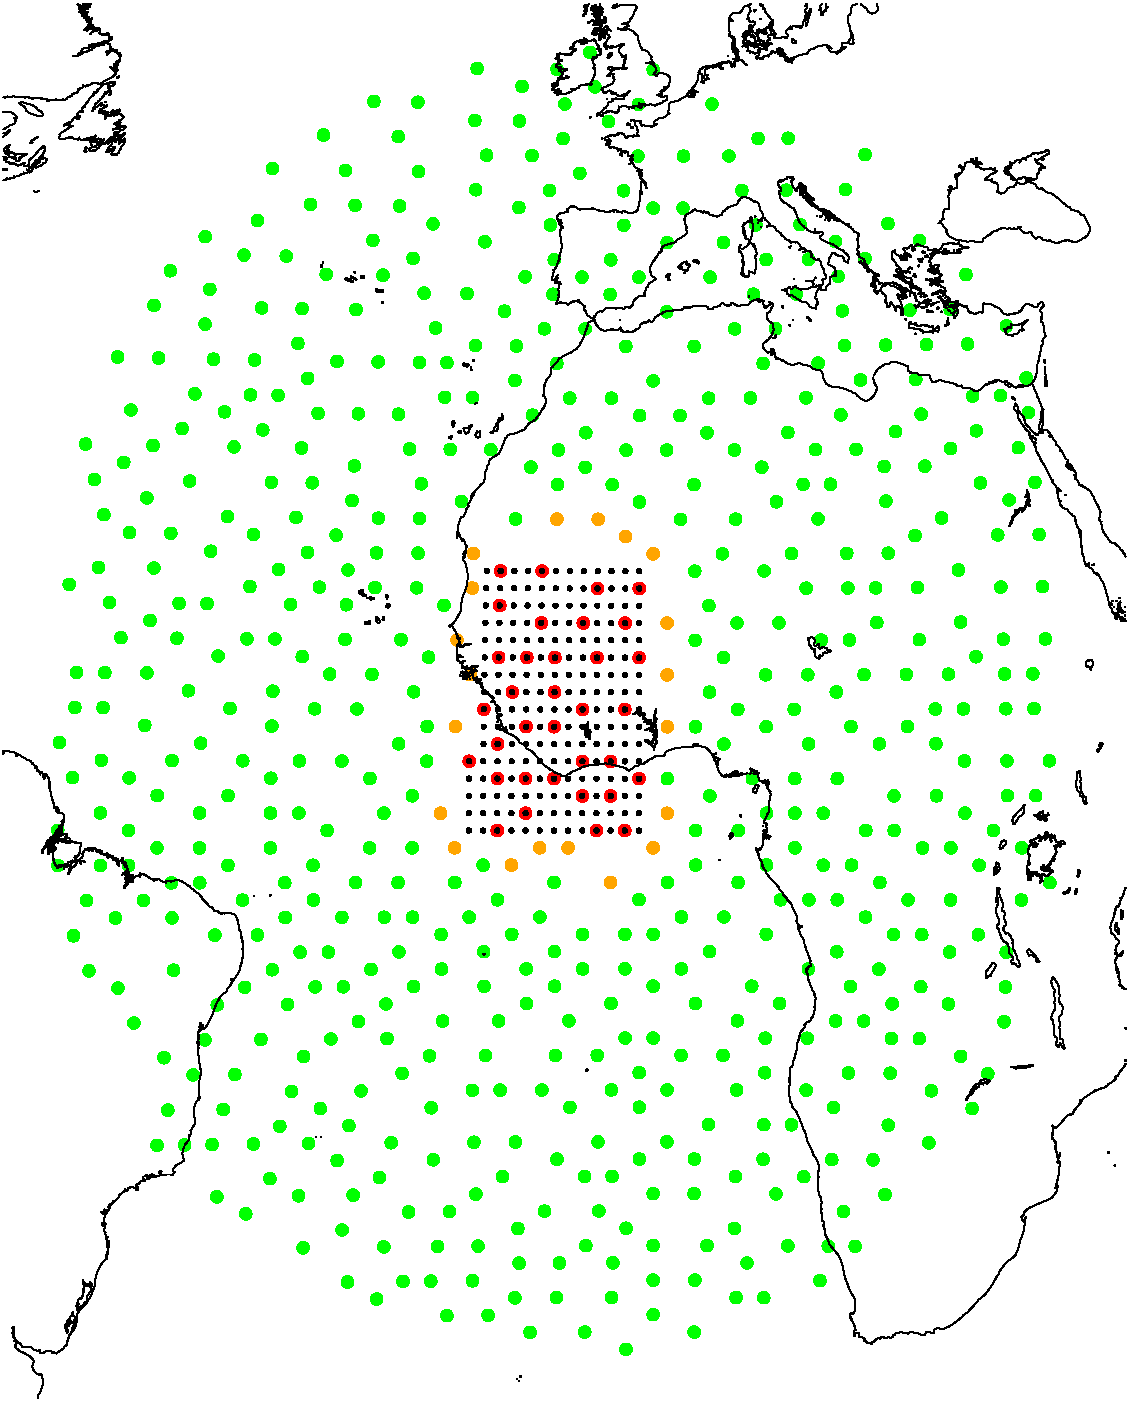
\includegraphics[height=0.6\linewidth]{arp_6B60_halo_1.pdf}
\captionof{figure}{On a given task: halo zones \textbf{[F]}, \textcolor{red}{\textbf{[A]}}, \textcolor{orange}{\textbf{[B]}} and \textcolor{green}{\textbf{[C]}} for the single communication method}
\end{center}

\subsection{Double communication method}
Another option is to add a communication step between the adjoint interpolation and the convolution, from halo zone \textbf{[B]} to halo zone \textbf{[A]}:
\begin{align}
\widetilde{\mathbf{C}} = \ _{\mathbf{[F]}} \ \mathbf{N} \ _{\mathbf{[F]}} \ \mathbf{S} \ _{\mathbf{[B]} \text{$\mathrlap{\boldsymbol{\leftarrow}}\boldsymbol{\prec}$} \mathbf{[A]} \text{$\mathrlap{\boldsymbol{\leftarrow}}\boldsymbol{\prec}$} \mathbf{[C]}} \ \mathbf{C}^s \ _{\mathbf{[C]} \boldsymbol{\leftarrow} \mathbf{[A]} \text{$\mathrlap{\boldsymbol{\leftarrow}}\boldsymbol{\prec}$} \mathbf{[B]}} \ \mathbf{S}^{\mathrm{T}} \ _{\mathbf{[F]}} \ \mathbf{N}^{\mathrm{T}} \ _{\mathbf{[F]}}
\end{align}
The nodes involved in the convolution are copied from halo zone \textbf{[A]} to halo zone \textbf{[C]} before the convolution. Thus, the halo zone \textbf{[C]} must include all the nodes involved in the convolution of nodes in the halo zone \textbf{[A]}.\\
$  $\\
The double communication method has an extra communication step, but the halo zone \textbf{[C]} is slightly reduced compared to the single communication method. Surprisingly, preliminary tests show that the double communication method is always faster than the single communication method.

\begin{center}
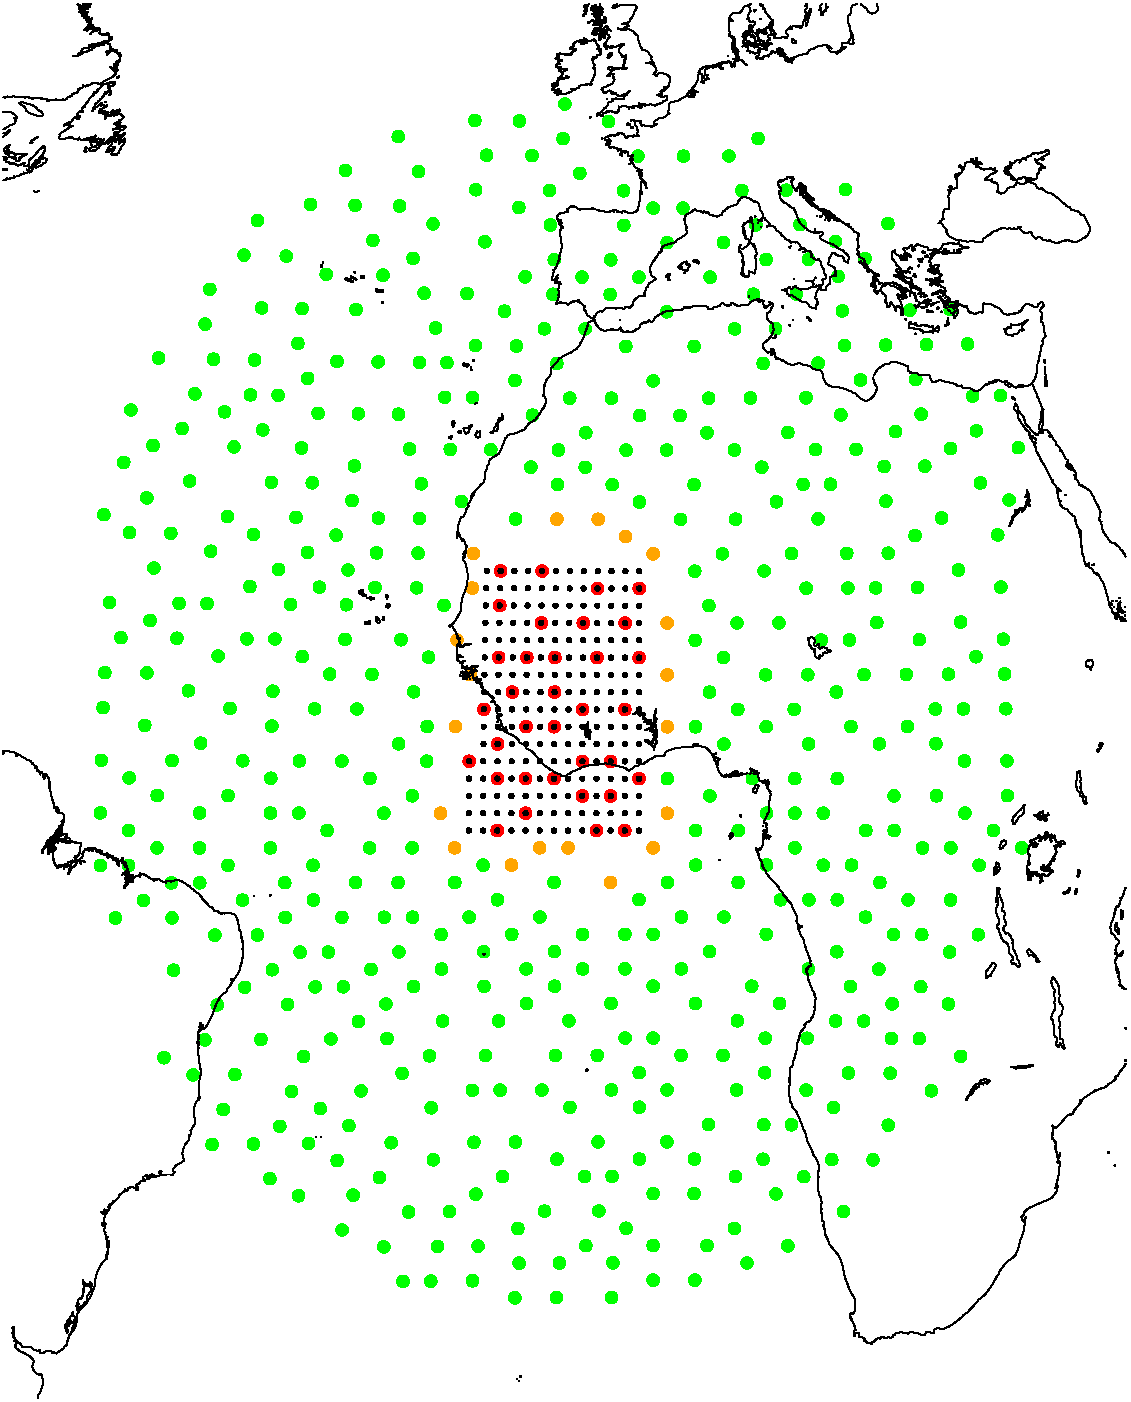
\includegraphics[height=0.6\linewidth]{arp_6B60_halo_2.pdf}
\captionof{figure}{On a given task: halo zones \textbf{[F]}, \textcolor{red}{\textbf{[A]}}, \textcolor{orange}{\textbf{[B]}} and \textcolor{green}{\textbf{[C]}} for the double communication method}
\end{center}

\section{Numerical efficiency}

\subsection{Theoretical computational cost}
The cost of the direct and adjoint interpolations is directly linked to the kind of horizontal and vertical interpolation used. In NICAS, we use a bilinear interpolation for the horizontal and a linear interpolation for the vertical:
\begin{itemize}
\item the number of operations in $\mathbf{S}^h$ is bounded by $3 n^c_0 n^l_0 = 3n$,
\item the number of operations in $\mathbf{S}^v$ is bounded by $2 n^l_0 n^c_1$,
\item the number of operations in $\mathbf{S}^s$ is bounded by $\displaystyle 3 \sum_{i^l \in \mathcal{S}^l_1} n^c_2(i^l) \le 3 n^c_1 n^l_1$
\end{itemize}
Thus, the dominant cost is in the horizontal interpolation $\mathbf{S}^h$, and the number of operations is bounded by $n^\mathrm{interp} = 3n$. In a parallel implementation with $p$ tasks, the cost per task becomes
\begin{align}
n^\mathrm{interp}_\mathrm{MPI} = 3 \frac{n}{p}
\end{align}
The interpolation cost is independent from the convolution parameters and is only proportional to the number of $\mathcal{G}^f$ nodes per task.\\
$  $\\
We can estimate the size of the subgrid $\mathcal{G}^s$ in the context of homogeneous support radii $r^h$ and $r^v$. Equation \ref{eq:nc} and \ref{eq:nl} lead to an approximate value of $n^s$:
\begin{align}
n^s = n^c n^l \approx \frac{2 \mathcal{V} \rho^3}{\sqrt{3} \left(r^h\right)^2 r^v}
\end{align}
where $\mathcal{V} = \mathcal{A} \mathcal{H}$ is the domain volume. The 3D compact support of the convolution function is an ellipsoid of volume:
\begin{align}
\mathcal{V}_\mathrm{cs} = \frac{4}{3} \pi \left(r^h\right)^2 r^v
\end{align}
Thus, $n^s$ can be expressed as:
\begin{align}
n^s = \frac{8 \pi}{3\sqrt{3}} \frac{\mathcal{V}}{\mathcal{V}_\mathrm{cs}} \rho^3
\end{align}
The density of nodes $\mathcal{D}$ is:
\begin{align}
\mathcal{D} = \frac{n_s}{\mathcal{V}} = \frac{8\pi}{3\sqrt{3}} \frac{\rho^3}{\mathcal{V}_\mathrm{cs}}
\end{align}
so the number of points in the 3D compact support of the convolution function is:
\begin{align}
m^s = \mathcal{D} \mathcal{V}_\mathrm{cs} = \frac{8\pi \rho^3}{3\sqrt{3}}
\end{align}
As a consequence, the number of operations for the convolution is approximately:
\begin{align}
n^\mathrm{convol} = n^s m^s = \frac{64\pi^2}{27} \frac{\mathcal{V}}{\mathcal{V}_\mathrm{cs}} \rho^6 = \frac{64\pi^2}{27} n \frac{v}{\mathcal{V}_\mathrm{cs}} \rho^6
\end{align}
where $v$ is the average volume of a cell of $\mathcal{G}^f$. In a parallel implementation with $p$ tasks, the cost per task becomes
\begin{align}
n^\mathrm{convol}_\mathrm{MPI} = \frac{64\pi^2}{27} \frac{n}{p} \frac{v}{\mathcal{V}_\mathrm{cs}} \rho^6
\end{align}
Thus, the convolution cost is proportional to:
\begin{itemize}
\item the number of $\mathcal{G}^f$ nodes per task,
\item the inverse of the ratio $\mathcal{V}_\mathrm{cs}/v$, which gives an indication of the convolution function support volume compared to a grid cell volume, i.e. the smoothing intensity of the convolution,
\item the resolution $\rho$ to the power 6.
\end{itemize}

\subsection{Theoretical communication cost}
We consider a parallel implementation with $p$ tasks where:
\begin{itemize}
\item all levels of a given column are handled by the same task,
\item each task handles points on a square of side $r_\mathbf{[A]}$ (area $\mathcal{A}_\mathbf{[A]} = r_\mathbf{[A]}^2$),
\item the repartition among tasks is even: $\mathcal{A}_\mathbf{[A]} = \mathcal{A}/p$
\item $p$ is large enough so that the halo zone \textbf{[C]} is not overlapping itself.
\end{itemize}
In this case, the area of the halo zone \textbf{[C]} is given by:
\begin{align}
\mathcal{A}_\mathbf{[C]} = \mathcal{A}_\mathbf{[A]} + 4 r_\mathbf{[A]} r^h + \pi\left(r^h\right)^2
\end{align}
so that the area in the halo zone \textbf{[C]} but not in the halo zone \textbf{[A]} is
\begin{align}
\overbar{\mathcal{A}_\mathbf{[C]}} & = \mathcal{A}_\mathbf{[C]} - \mathcal{A}_\mathbf{[A]} = 4 r_\mathbf{[A]} r^h + \pi\left(r^h\right)^2
\end{align}
Thus, the number of communications between the halo zone \textbf{[C]} and the halo zone \textbf{[A]}, which is approximately equal to the number of points in the volume $\overbar{\mathcal{V}_\mathbf{[C]}} = \overbar{\mathcal{A}_\mathbf{[C]}} \mathcal{H}$, is given by:
\begin{align}
\label{eq:ncom}
n_\mathrm{com} & = \mathcal{D} \overbar{\mathcal{V}_\mathbf{[C]}} \nonumber \\
& = \frac{8\pi}{3\sqrt{3}} \frac{\rho^3}{\mathcal{V}_\mathrm{cs}} \left(4 r_\mathbf{[A]} r^h + \pi\left(r^h\right)^2\right) \mathcal{H} \nonumber \\
& =  \frac{4\pi}{\sqrt{3}} \rho^2 n^l \left(\sqrt{\frac{p_\mathrm{lim}}{p}} +1 \right)
\end{align}
where
\begin{align}
p_\mathrm{lim} = \frac{16 \mathcal{A}}{\pi^2 \left(r^h\right)^2}
\end{align}
For instance in a global model:
\begin{itemize}
\item with a support radius $r^h$ = 2000 km, $p_\mathrm{lim} \approx 207$,
\item with a support radius $r^h$ = 1000 km, $p_\mathrm{lim} \approx 826$,
\item with a support radius $r^h$ = 500 km, $p_\mathrm{lim} \approx 3307$.
\end{itemize}
We notice, as expected, that the number of communications $n_\mathrm{com}$ is proportional to the number of levels $n^l$ in the subgrid, and to the resolution $\rho$ squared. If $p \ll p_\mathrm{lim}$, then $n_\mathrm{com}$ is also proportional to the inverse square-root of $p$.\\
$  $\\
A key aspect of the NICAS method is that communications are performed on the subgrid $\mathcal{G}^s$ and do not depend explicitly on the size of the full grid $\mathcal{G}^f$. However in the present implementation, the distribution of $\mathcal{G}^s$ points among tasks is still defined from the distribution of $\mathcal{G}^f$ points, which can introduce imbalances in the tasks load.

\subsection{Resolution impact}
The resolution parameter has been introduced to compute the subgrid size. Figures \ref{fig:resol_8}, \ref{fig:resol_6} and \ref{fig:resol_4} show the decrease of subgrid density with the resolution parameter.

\begin{center}
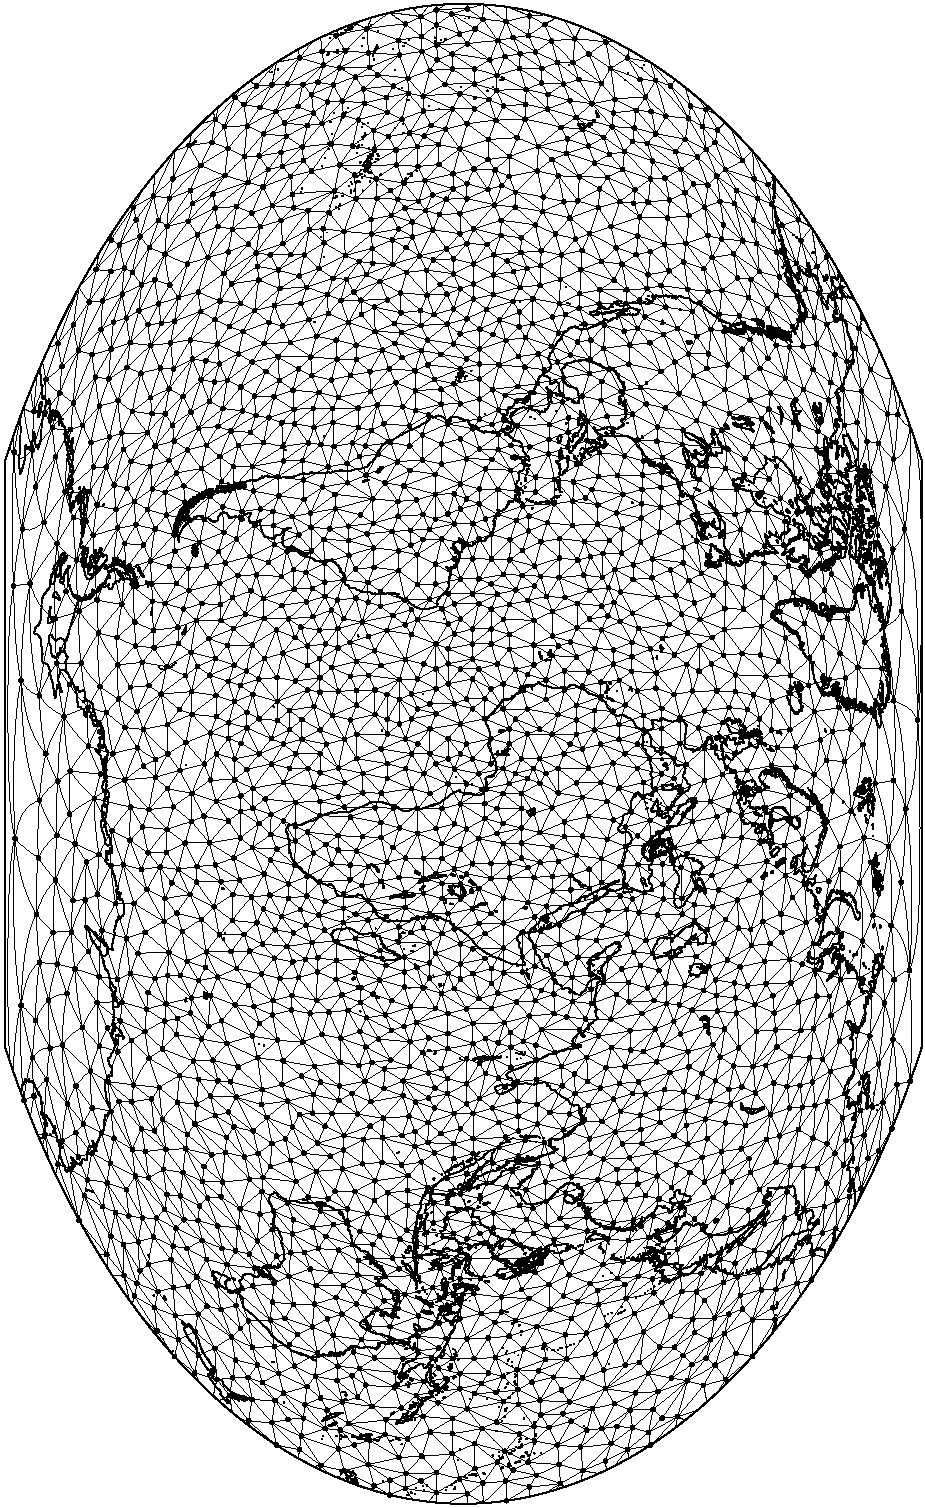
\includegraphics[height=0.75\linewidth,angle=90]{arp_6B60_mesh_001_resol-8.pdf}
\captionof{figure}{Subgrid $\mathcal{S}^c_1$ with a resolution parameter $\rho = 8$ ($n^c_1 = 2827$) \label{fig:resol_8}}
\end{center}
\begin{center}
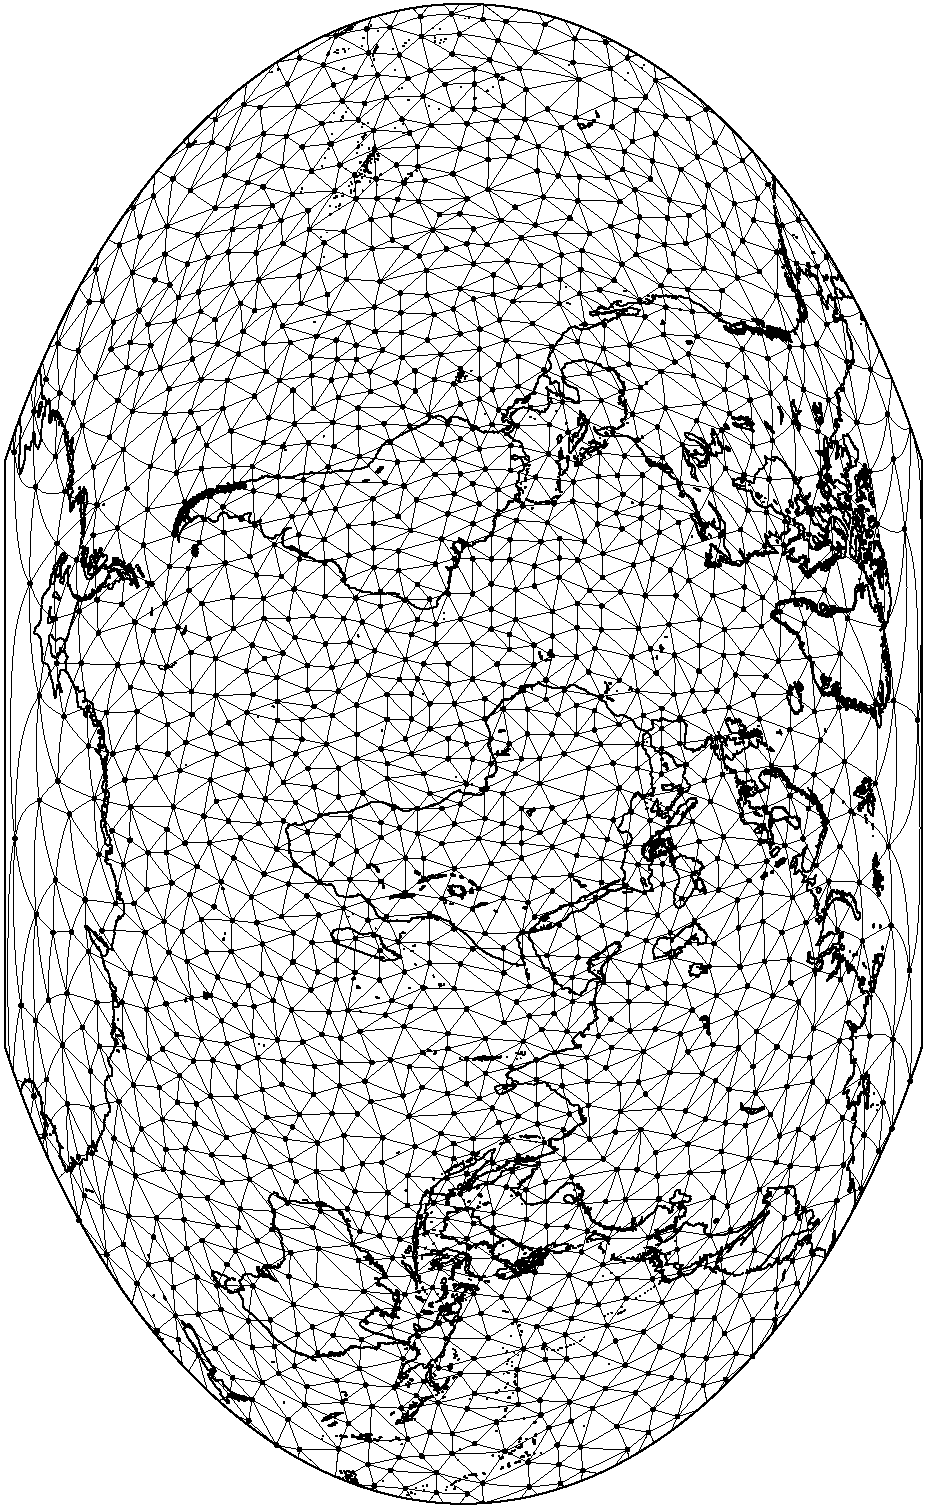
\includegraphics[height=0.75\linewidth,angle=90]{arp_6B60_mesh_001_resol-6.pdf}
\captionof{figure}{Subgrid $\mathcal{S}^c_1$ with a resolution parameter $\rho = 6$ ($n^c_1 = 1590$) \label{fig:resol_6}}
\end{center}
\begin{center}
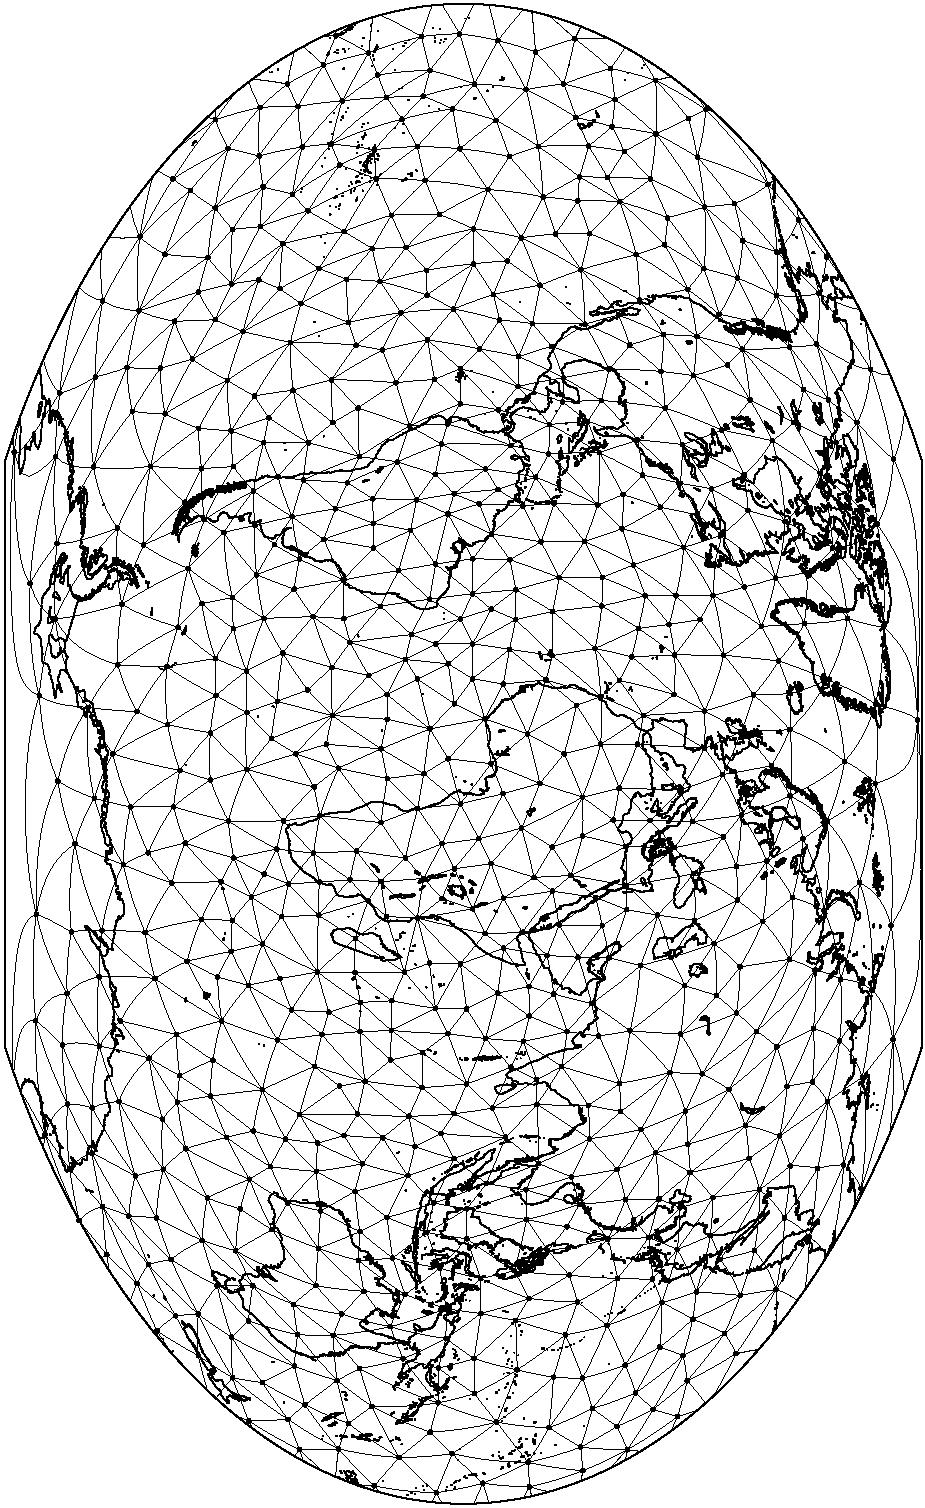
\includegraphics[height=0.75\linewidth,angle=90]{arp_6B60_mesh_001_resol-4.pdf}
\captionof{figure}{Subgrid $\mathcal{S}^c_1$ with a resolution parameter $\rho = 4$ ($n^c_1 = 706$) \label{fig:resol_4}}
\end{center}

A coarser grid results in larger interpolation errors, so that the convolution function on the full grid $\mathcal{S}^f$ looks more "bumpy". Figures \ref{fig:localization_arp} and \ref{fig:localization_ver_arp} show a comparison of convolution functions for a spectral method and for the NICAS method with a decreasing resolution.

\begin{center}
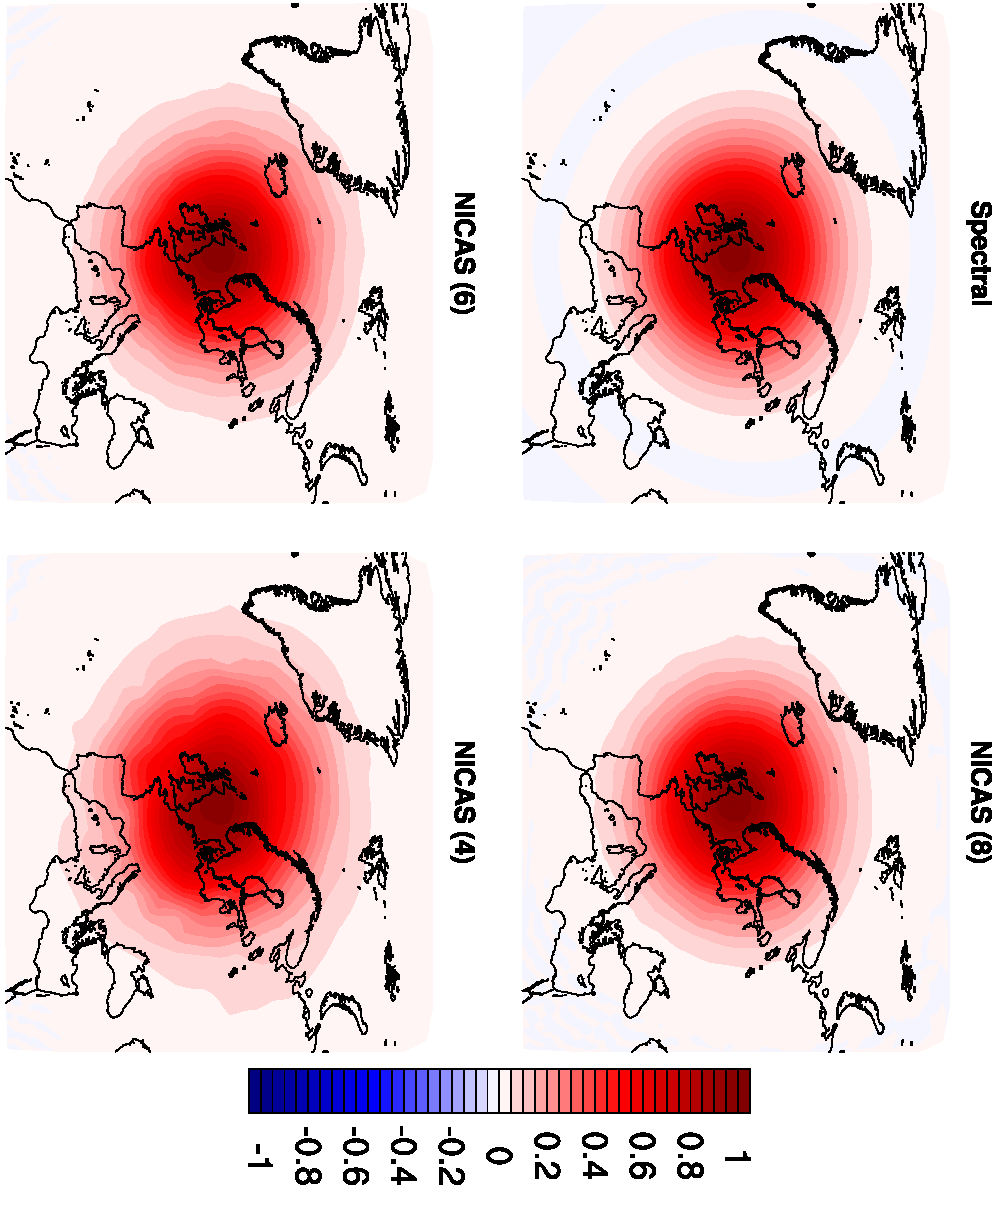
\includegraphics[height=0.8\linewidth,angle=90]{localization_arp.pdf}
\captionof{figure}{Horizontal convolution function for a spectral method and for the NICAS method with a decreasing resolution ($\rho$ = 8, 6 and 4). \label{fig:localization_arp}}
\end{center}
\begin{center}
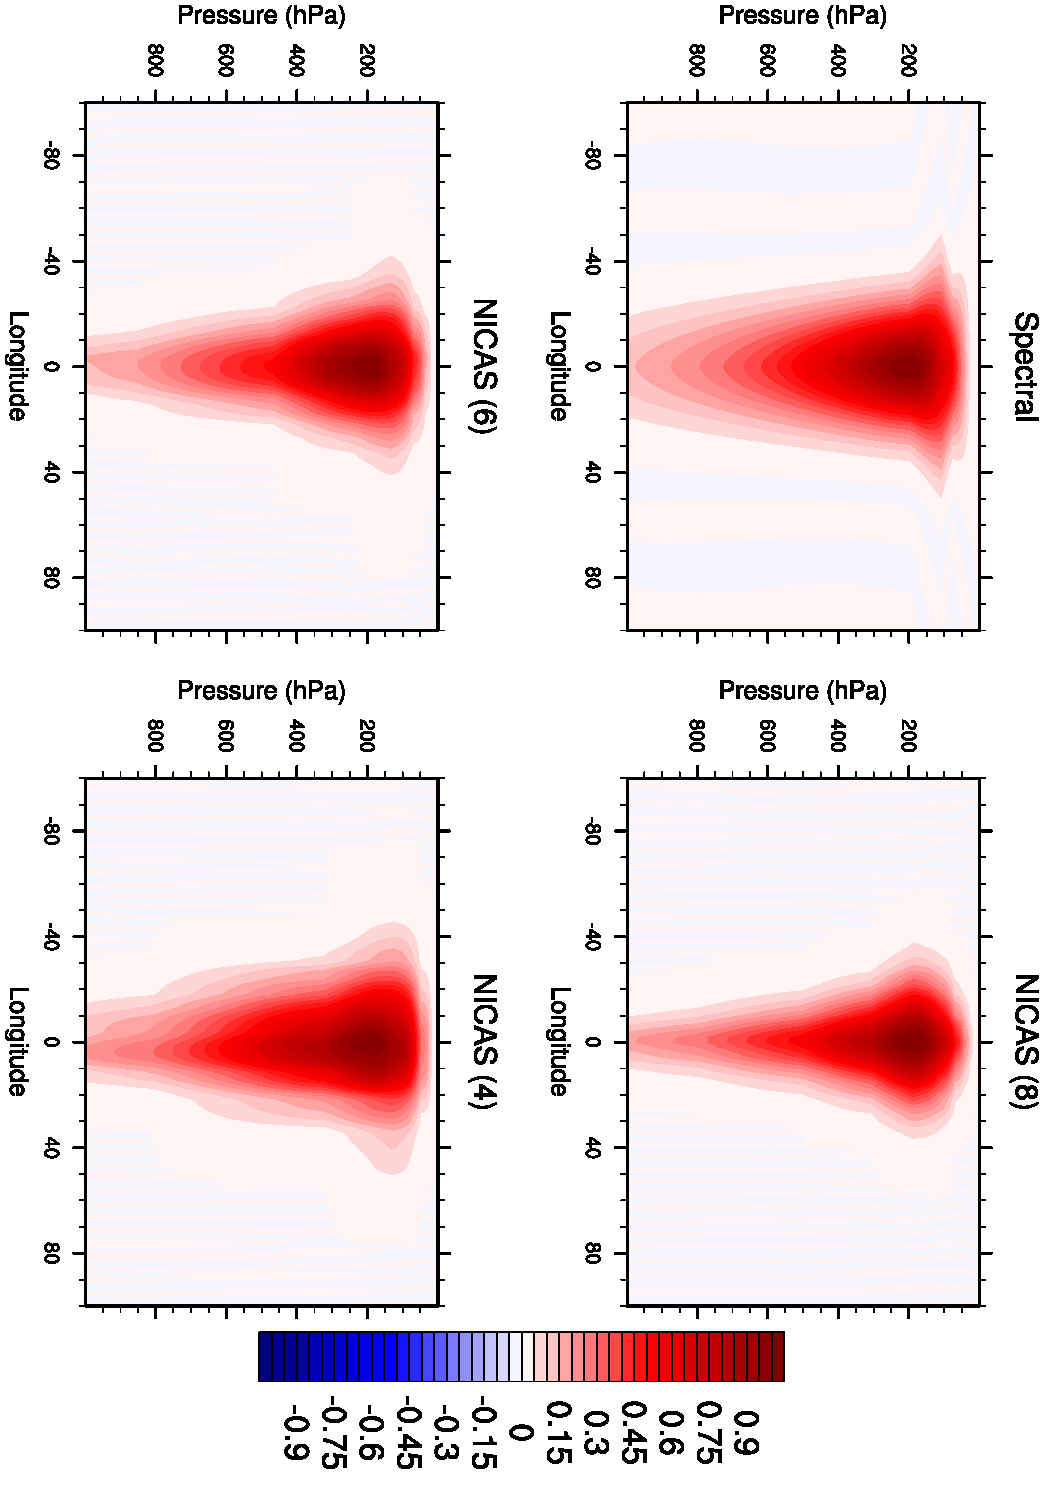
\includegraphics[height=0.8\linewidth,angle=90]{localization_ver_arp.pdf}
\captionof{figure}{Vertical convolution function for a spectral method and for the NICAS method with a decreasing resolution ($\rho$ = 8, 6 and 4). \label{fig:localization_ver_arp}}
\end{center}

\bibliographystyle{mybib-en}
\bibliography{nicas}

\end{document}
